\section{3Dプリンタの基本原理}\label{dux30d7ux30eaux30f3ux30bfux306eux57faux672cux539fux7406}

3Dプリンタには下記のように様々な方式があります。

\begin{itemize}
\tightlist
\item
  熱溶解積層法 FDM (Fused Deposition Modeling)
\item
  光造形方式 STL (STereo Lithography)
\item
  インクジェット粉末積層方式
\item
  粉末焼結方式 SLS法(Selective Laser Sintering)
\end{itemize}

家庭用として売られているものの多くは1番上の熱溶解積層法の3Dプリンタです。
以下、 熱溶解積層法の3Dプリンタについて簡単に解説していきます。

\subsection{熱溶解積層法(FDM)}\label{ux71b1ux6eb6ux89e3ux7a4dux5c64ux6cd5fdm}

熱溶解積層法(FDM)の基本原理をFig.\ref{fig22}に示します。

Fig.\ref{fig22}に示した通り、熱で溶かした樹脂をテーブルの上に積層していくことで形状を作っていきます。
生クリームを絞り出していく様子をイメージしてもらえると分かりやすいかと思います。 

使用する樹脂は「フィラメント」と呼ばれ、細い線形状をしています。
多くの場合、「スプール(糸巻き)」に巻き付けられて販売されています。

このスプールを3Dプリンタ本体へ取り付け、フィラメントの先端を「ノズル」に取り付けます。
ノズルにはモータと加熱部が搭載されており、必要な分だけフィラメントを引張り出し、溶かしながらテーブルへと吐出していきます。

吐出を続けながら、ノズル・テーブルがXYZに動くことで、形状が作られていきます。
ノズルやテーブルの動き方は、3Dプリンタの構造によって異なります。

\begin{figure}[htbp]
\centering
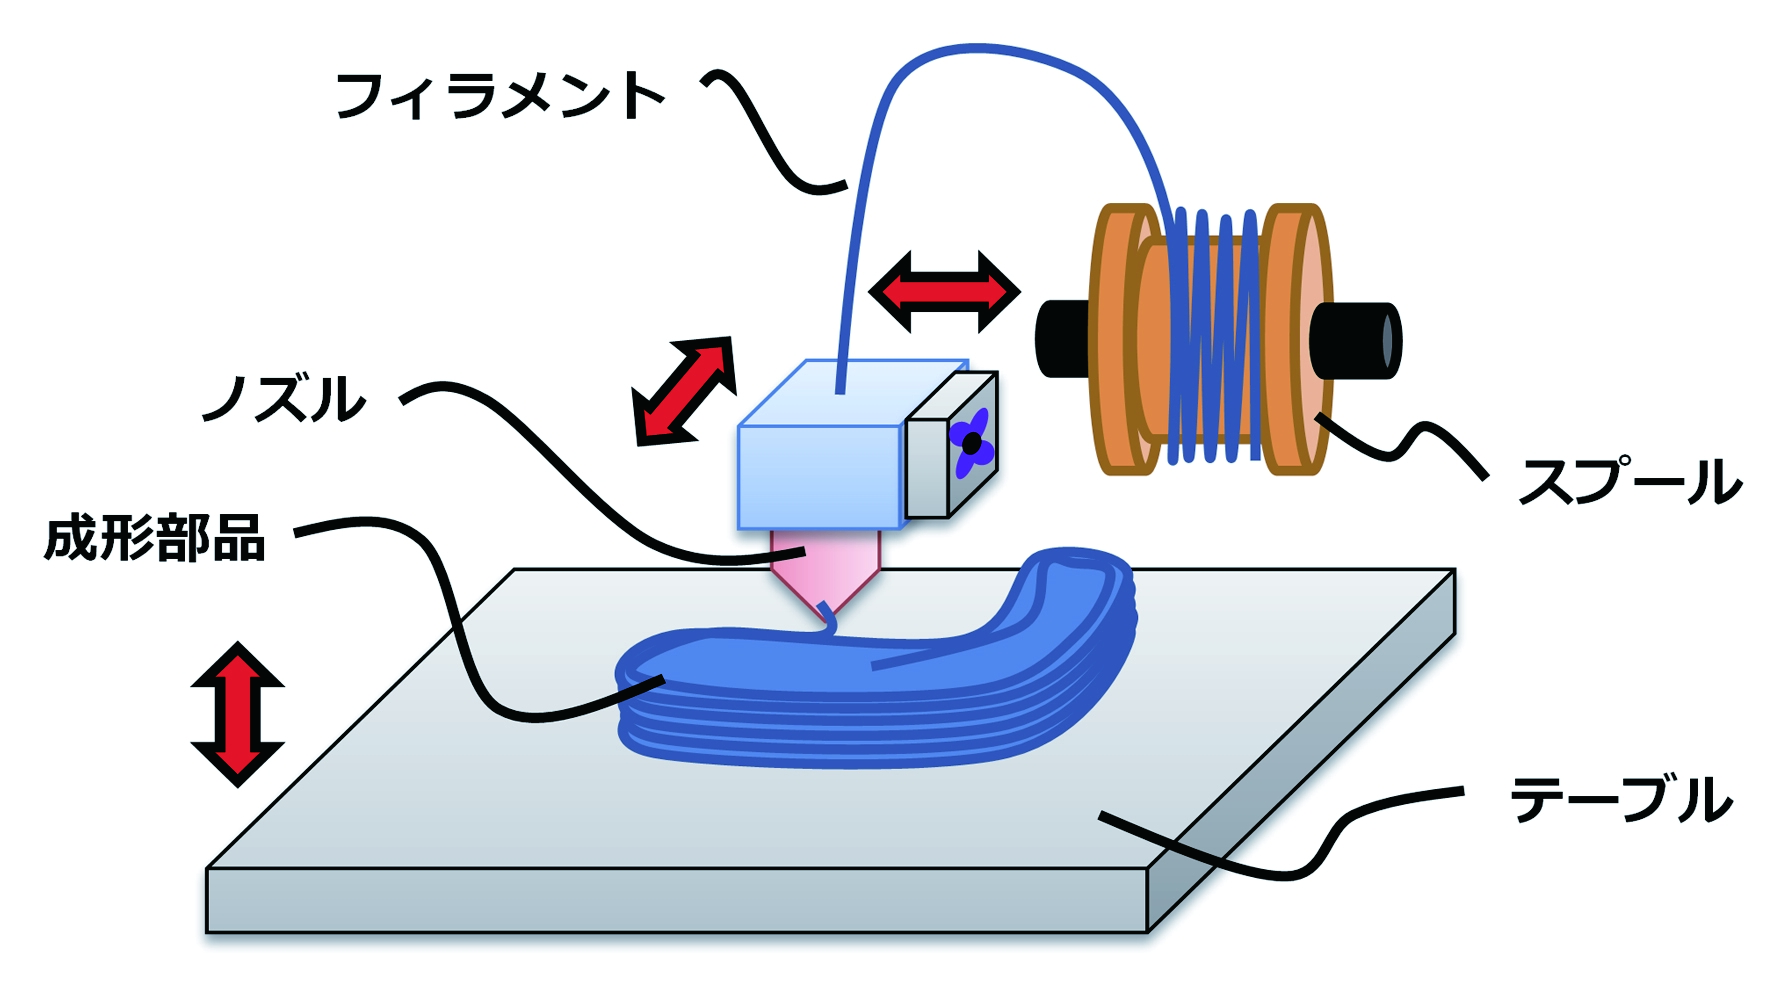
\includegraphics[width=300pt]{fig/fig22_cmyk.jpg}
\caption{熱溶解積層方式(FDM)の原理}
\label{fig22}
\end{figure}

\subsection{熱溶解積層方法の特徴}\label{ux71b1ux6eb6ux89e3ux7a4dux5c64ux65b9ux6cd5ux306eux7279ux5fb4}

熱溶解積層方法の3Dプリンタは下記のような特徴を持っています。

\subsubsection{長所}\label{ux9577ux6240}

\begin{itemize}
\tightlist
\item
  他方式の3Dプリンタより安価(本体・材料ともに)
\item
  使用できる材料の種類が豊富(材料種類・カラーが豊富)
\item
  樹脂を用いる3Dプリンタの中では、他の方式より比較的強い部品が作れる
\item
  3Dモデルだけで部品を作ることができる(2D図面が不要)
\end{itemize}

\subsubsection{短所}\label{ux77edux6240}

\begin{itemize}
\tightlist
\item
  原理的に寸法精度が切削加工ほど良くない(大凡0.1mmオーダー)
\item
  表面が荒い(側面に積層ピッチに応じた段差ができる)
\item
  衝撃や強い力が加わると積層面から剥がれることがある
\item
  成形時に部品に反りが発生することがある
\item
  大きな部品を作ると、時間がかかる(※製品によります)
\end{itemize}

\clearpage

\section{3Dプリンタの基本的な構造}\label{dux30d7ux30eaux30f3ux30bfux306eux57faux672cux7684ux306aux69cbux9020}

3Dプリンタの構造には大きく分けて以下の4つがあります。
図\ref{fig23}に構造別の長所・短所、製品例を挙げます。
因みにBOX型の製品例である「Replicator
2x(MakerBot社)」が私が持っている製品です。

\begin{itemize}
\tightlist
\item
  メンデル型
\item
  フレーム型
\item
  BOX型
\item
  ROSTOCK型
\end{itemize}

\begin{figure}[htbp]
\centering
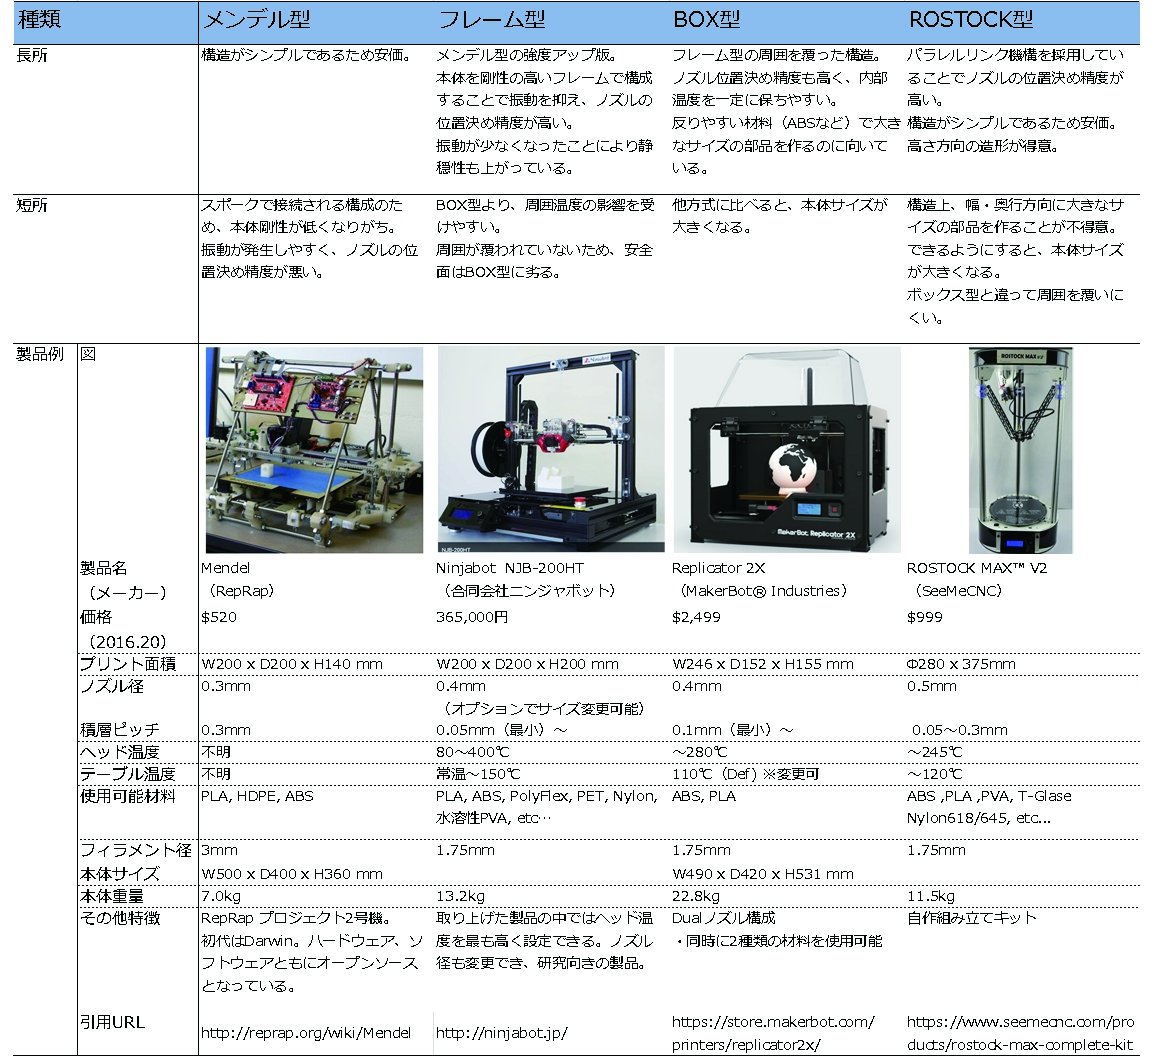
\includegraphics[width=380pt]{fig/fig23_cmyk.jpg}
\caption{3Dプリンタの構造}
\label{fig23}
\end{figure}

\section{3Dプリンタの選定}\label{dux30d7ux30eaux30f3ux30bfux306eux9078ux5b9a}

私が3Dプリンタを購入した当時(2013年)は選択肢が少なかったですが、2016年現在では非常に多くの製品が出ています。
前述したように3Dプリンタには短所も多いため、下記のような観点から自分に適した製品を選択する必要があります。

\begin{itemize}
\tightlist
\item
  使用材料・部品サイズ
\item
  寸法精度・外観
\item
  ユーザビリティ
\end{itemize}

\subsection{使用材料・部品サイズ}\label{ux4f7fux7528ux6750ux6599ux90e8ux54c1ux30b5ux30a4ux30ba}

3Dプリンタの代表的な造形材料はPLAとABSです。
特徴はFig.\ref{fig31}の通りです。

\begin{figure}[htbp]
\centering
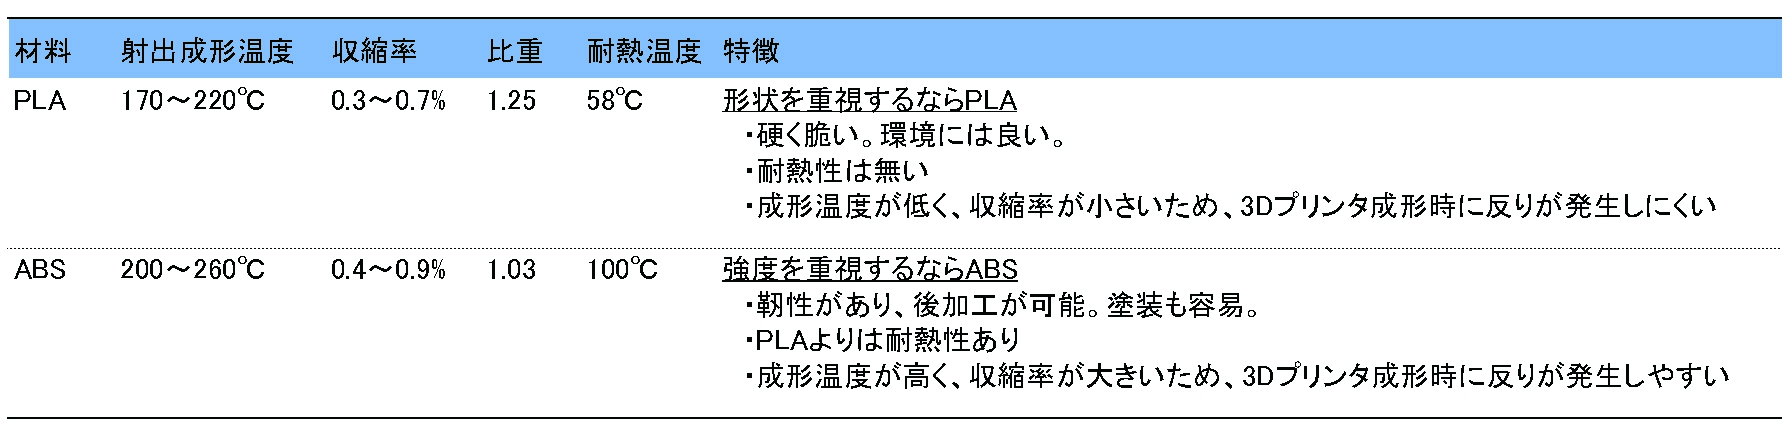
\includegraphics[width=360pt]{fig/fig31_cmyk.jpg}
\caption{代表的な造形材料と特徴}
\label{fig31}
\end{figure}

PLAよりもABSの方が成形が困難だと言われています。
ABSはPLAより収縮率が大きく、収縮力で最下層面とテーブルが剥がれ、部品に反りが出やすいためです。
(Fig.\ref{fig32})

\begin{figure}[htbp]
\centering
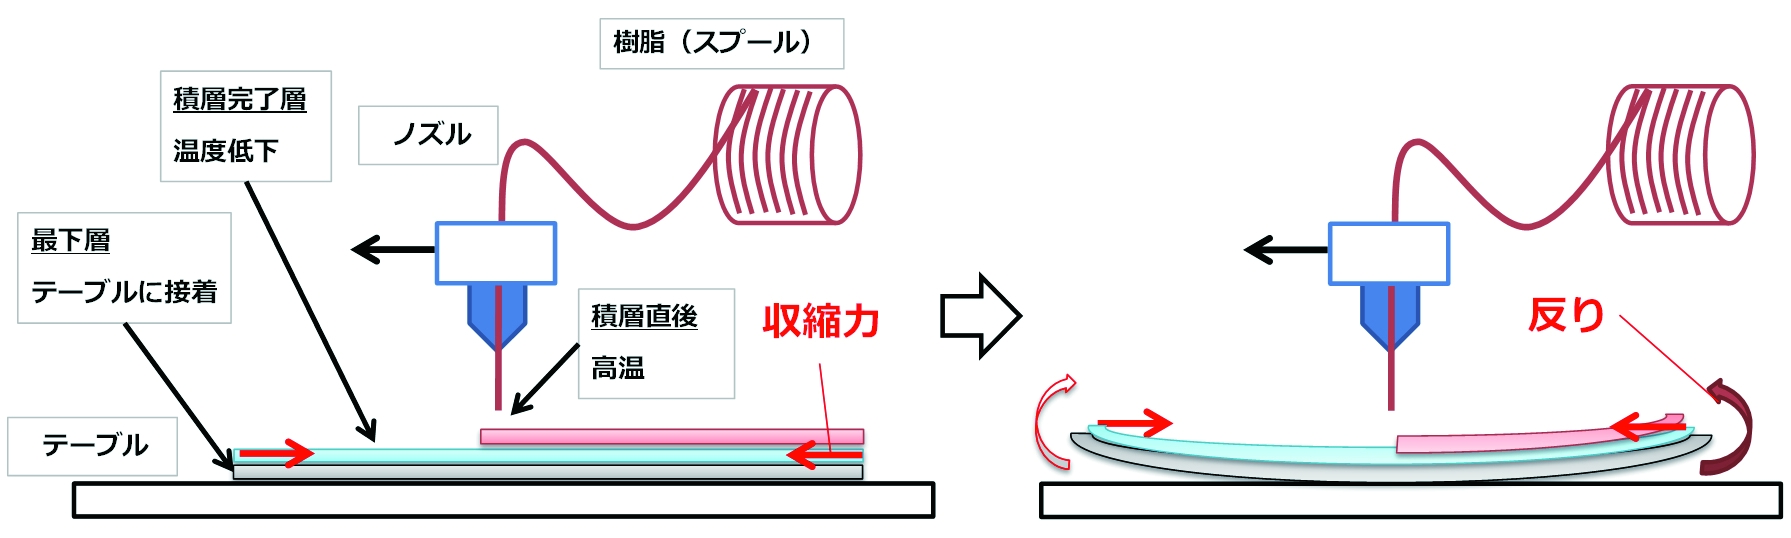
\includegraphics[width=380pt]{fig/fig32_cmyk.jpg}
\caption{反りの発生原理}
\label{fig32}
\end{figure}

よって、ABSをメインで使いたい場合は、ボックス型、かつ反り対策が入った製品がよいでしょう。
但し、部品サイズが小さければ(□100mm以下)、安価なフレーム型でも反りを出さずに部品を作ることが可能です。

\subsubsection{\texorpdfstring{製品例1:UP Plus(3D Systems
Inc.) ※Fig.\ref{fig28}
No.17}{製品例1:UP Plus(3D Systems Inc.) ※Fig. No.17}}\label{ux88fdux54c1ux4f8b1up-plus3d-systems-inc.fig.-no.17}

\begin{itemize}
\tightlist
\item
  □140mmまで対応したフレーム型3Dプリンタで、ABSに対応しています。
\item
  テーブル非加熱式のフレーム型のため熱が逃げやすい構成ですが、
  テーブルに細かい穴が空いており最下層の樹脂が穴に食い込むことで剥がれにくい対策を取っています。
\end{itemize}

因みに、同メーカから2016年に「UP BOX+」という後継機が出ています。
プリントサイズは□120mmまでと小さくなっていますが、ボックス型のため、反りがでにくそうです。

□150mmを大きく超えるサイズの部品をABSで作る場合には、以下のような積極的に反りを抑制する工夫が入った製品をお勧めします。

\subsubsection{\texorpdfstring{製品例2:Zortrax M200(Zortrax)
 ※Fig.\ref{fig26}
No.10}{製品例2:Zortrax M200(Zortrax)  ※Fig. No.10}}\label{ux88fdux54c1ux4f8b2zortrax-m200zortrax-fig.-no.10}

\begin{itemize}
\tightlist
\item
  □200mmまで対応したボックス型3Dプリンタで、ABSに対応しています。
\item
  テーブル加熱式、かつボックス型のため熱が逃げにくい構成となっており、成形安定性に定評があります。
\end{itemize}

\subsubsection{フィラメント径}\label{ux30d5ux30a3ux30e9ux30e1ux30f3ux30c8ux5f84}

フィラメント径はΦ1.75,
Φ3mmの2種類がありますが、現在はΦ1.75mmが主流です。

フィラメントは非正規品も多く出ていますが、品質が悪いものもあるのでご注意ください。
1kg3000円程度とコストは魅力的ですが、問題が発生することも多々あります。
例えば、フィラメントの線径にばらつきがあると部品形状にもムラができたり、最悪ノズルが詰まって成形に失敗することもあります。

\subsubsection{特殊フィラメント}\label{ux7279ux6b8aux30d5ux30a3ux30e9ux30e1ux30f3ux30c8}

フィラメントの材料は以前はABSとPLAが主流でしたが、近年は様々な種類が出ています。

例えば、アメリカのNinjatekが開発したNijaflex\cite{ninjaflex}はポリウレタン系の熱可塑性エラストマー(TPE)という材料です。
プラスチックとゴムの中間材料であるため、弾性を有していることが特徴です(ショア硬さ:85A)。
1kg10000円程度で購入可能です(2016.12月現在)。

また、アメリカのMakerBoが開発した\}TOUGH
PLA\cite{tough-pla}はPLAであるものの、耐久性と衝撃強度に優れた材料になっています。
750g 6000円程度で購入可能です(2016.12月現在)。
物性値は下記の通りです。

\begin{itemize}
\tightlist
\item
  ABS\ldots{}\ldots{}曲げ強さ:79MPa, 曲げ弾性率:2669MPa
\item
  TOUGH PLA\ldots{}\ldots{}曲げ強さ:63MPa, 曲げ弾性率:2366MPa
\end{itemize}

その他にも、HIPS(耐衝撃性ポリスチレン)、NYL(ナイロン)、CON(導電性フィラメント)、PVA(水溶性ポリビニルアルコール)、ガラスフィラー入り材料、等々続々と使用できる材料が増えてきています。
樹脂を溶融させて再度固める、という点では射出成型と原理は同じなので、理屈では材料も同じものが使えます。
勿論ABSで発生する反りなどは3Dプリンタ特有の問題なので、既存の材料を3Dプリンタ向けにアレンジする必要はあるかと思いますが、今後も使える材料は増えていくと思われます。

尚、材料の溶融温度は樹脂材料によって決まりますので、ノズルの最高温度が高く、かつ自由に設定できる製品であるほど使用できる材料の幅が広くなると思います。
将来に材料が増えることに期待して、ノズル温度を高くできる製品を選択するというのもありかもしれませんね。

\subsubsection{\texorpdfstring{製品例3:Ninjabot
NJB-200HT(合同株式会社ニンジャボット)
 ※Fig.\ref{fig23}}{製品例3:Ninjabot NJB-200HT(合同株式会社ニンジャボット)  ※Fig.}}\label{ux88fdux54c1ux4f8b3ninjabot-njb-200htux5408ux540cux682aux5f0fux4f1aux793eux30cbux30f3ux30b8ux30e3ux30dcux30c3ux30c8-fig.}

\begin{itemize}
\tightlist
\item
  樹脂の可能性そのものを研究する目的で開発されたフレーム型3Dプリンタです。
\item
  テーブルは150℃まで加熱でき、ノズルも、80~400℃と低温から高温までカバーしています。
\end{itemize}

\subsection{寸法精度・外観}\label{ux5bf8ux6cd5ux7cbeux5ea6ux5916ux89b3}

寸法精度・外観に影響を与える項目は前述した「反り」の他に下記項目があげられます。

\begin{itemize}
\tightlist
\item
  位置決め精度
\item
  積層ピッチ
\end{itemize}

テーブル・ノズルの位置決め精度が寸法精度・外観へ影響を与えます。
また、剛性が弱い3Dプリンタでは振動による精度ばらつきが追加されます。

積層ピッチに関しては、小さいほど積層跡が目立たなくなり、外観は綺麗にできます。
但し、積層ピッチが小さいと成形に失敗しやすくなります。
樹脂を積層する際に、積層ピッチ以上に位置決めの精度がばらつくと、積層界面で樹脂が溶着しなくなるためです。

世の中の3Dプリンタを見ると、剛性が高く精度の高い3Dプリンタほど、積層ピッチが小さくなっています。

\subsection{ユーザビリティ}\label{ux30e6ux30fcux30b6ux30d3ux30eaux30c6ux30a3}

3Dプリンタはいまだ発展途上の製品のため、ユーザが調整作業やメンテナンスをすることが多いです。
3Dプリンタの構造や搭載されている機能によって、ユーザの負荷が変わりますので、選定の際にはユーザビリティを考慮する必要があるでしょう。

\subsubsection{ノズル高さ自動調整機能}\label{ux30ceux30baux30ebux9ad8ux3055ux81eaux52d5ux8abfux6574ux6a5fux80fd}

3Dプリンタの部品の出来具合を左右する要因の一つに、ノズルとテーブルの隙間量(Z方向)があります。
狭すぎるとノズルが樹脂が出てこずノズル詰まりの原因となります。
逆に広すぎると溶かした樹脂がテーブルに貼りつかず、成形失敗の原因となります。

自動調節機能が無い機種では、ノズル~テーブルの間に紙1枚(≒0.3mm)を通過させ、隙間量を手動調整することが多いです。
一方、ノズル高さ自動調整機能 (Fig.\ref{fig33}
(a))があると、成形前にノズル~テーブル間距離を自動で測定し、適切な隙間量に設定してくれます。

\subsubsection{テーブル傾き対応}\label{ux30c6ux30fcux30d6ux30ebux50beux304dux5bfeux5fdc}

ノズルの高さ自動調整機能を有した製品は数多くあっても、テーブルの傾きを物理的に補正する製品は殆どありません。
メカ機構が複雑になるからだと思われます。テーブル傾きの対応は製品ごとに様々です。

例えば、ノズル~テーブル間距離を測定する機能を持った製品の中には、テーブル上の4隅と中央の隙間を測定し、
どの程度調整すればよいか明示してくれるものもあります。この値をもとにユーザが手動調整します。

ノズル~テーブル高さの隙間測定機能を利用して、テーブル傾きに対応(Z軸オートキャリブレーション)した製品もあります。
最下層のサポート材の厚みで調整するタイプと、ノズルがテーブルの傾きに合わせて動くタイプ(Fig.\ref{fig33}
(b))、と2タイプあります。

\begin{figure}[htbp]
\centering
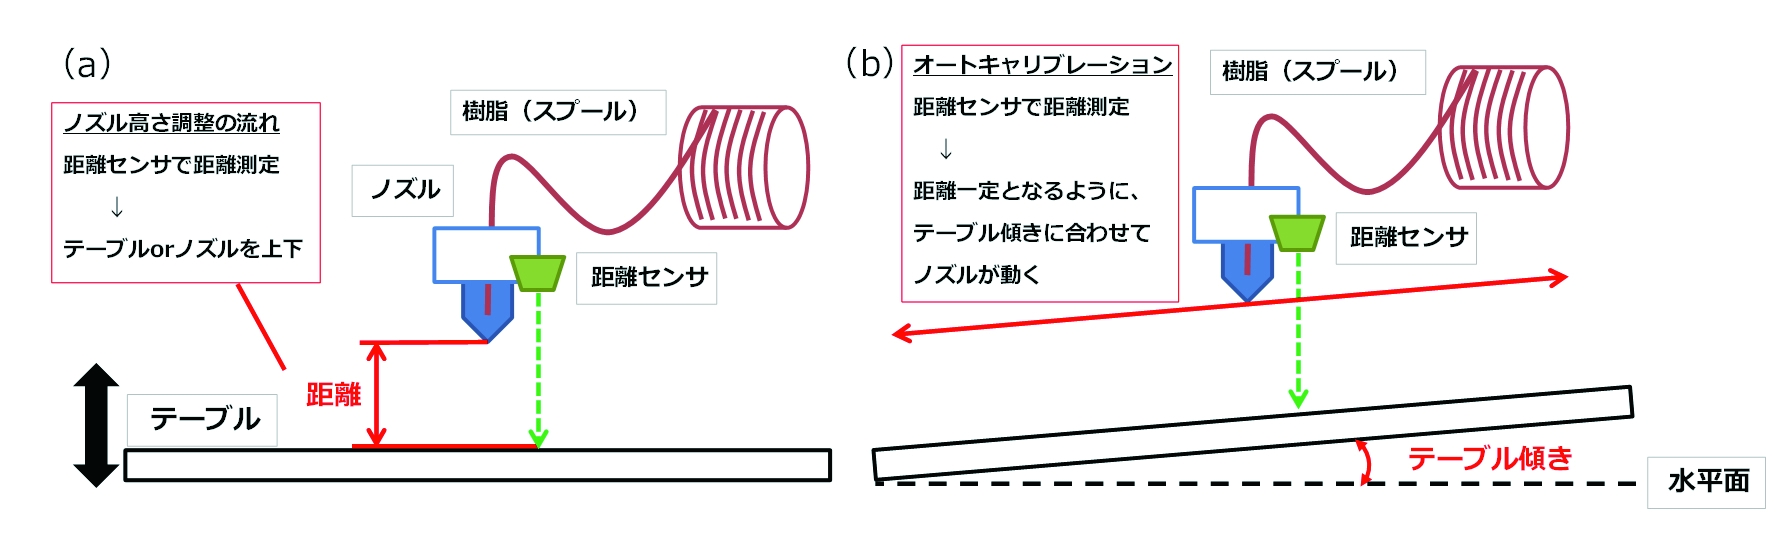
\includegraphics[width=380pt]{fig/fig33_cmyk.jpg}
\caption{ノズル高さ自動調節機能 / テーブル傾き対応}
\label{fig33}
\end{figure}

\subsection{コスト}\label{ux30b3ux30b9ux30c8}

コストには下記2つあります。

\begin{itemize}
\tightlist
\item
  本体価格
\item
  ランニングコスト
\end{itemize}

\subsubsection{本体価格}\label{ux672cux4f53ux4fa1ux683c}

本体価格は、Mendel型が最も安価です。
しかし、部品寸法精度や外観の観点から、あまりお勧めはしません。

2016年現在はそもそもMendel型のモデルは少なくなり、BOX型のモデルが充実してきています。
今後はROSTOCK型も増えていくでしょう。

10万~50万円くらいで幅広いラインナップが揃っていますので、
まずは最低限必要な機能を絞り、お財布と相談しながら候補を絞り込んでいくのがよいでしょう。

\subsubsection{ランニングコスト}\label{ux30e9ux30f3ux30cbux30f3ux30b0ux30b3ux30b9ux30c8}

ランニングコストに最も影響を与えるのが材料費用でしょう。

前述した通り、3Dプリンタは発展途上の製品なのでできるだけ純正フィラメントを使うことをお勧めします。
純正フィラメントの価格はメーカによって幅があります。
普通のABS樹脂ですと、純正品なら1kg 5000~6000円程度、非純正品なら1kg
3000円程度です。

1kgといっても、3Dプリンタの多くは部品の内側の充填率を下げて成形もできるので結構長持ちします。

尚、Cubeシリーズはやや高めの価格設定となっていますので、ランニングコストを気にされる方はご注意ください。

\section{3Dプリンタ一覧}\label{dux30d7ux30eaux30f3ux30bfux4e00ux89a7}

次ページから3Dプリンタの一覧を示します。

\clearpage

\begin{figure}[htbp]
\centering
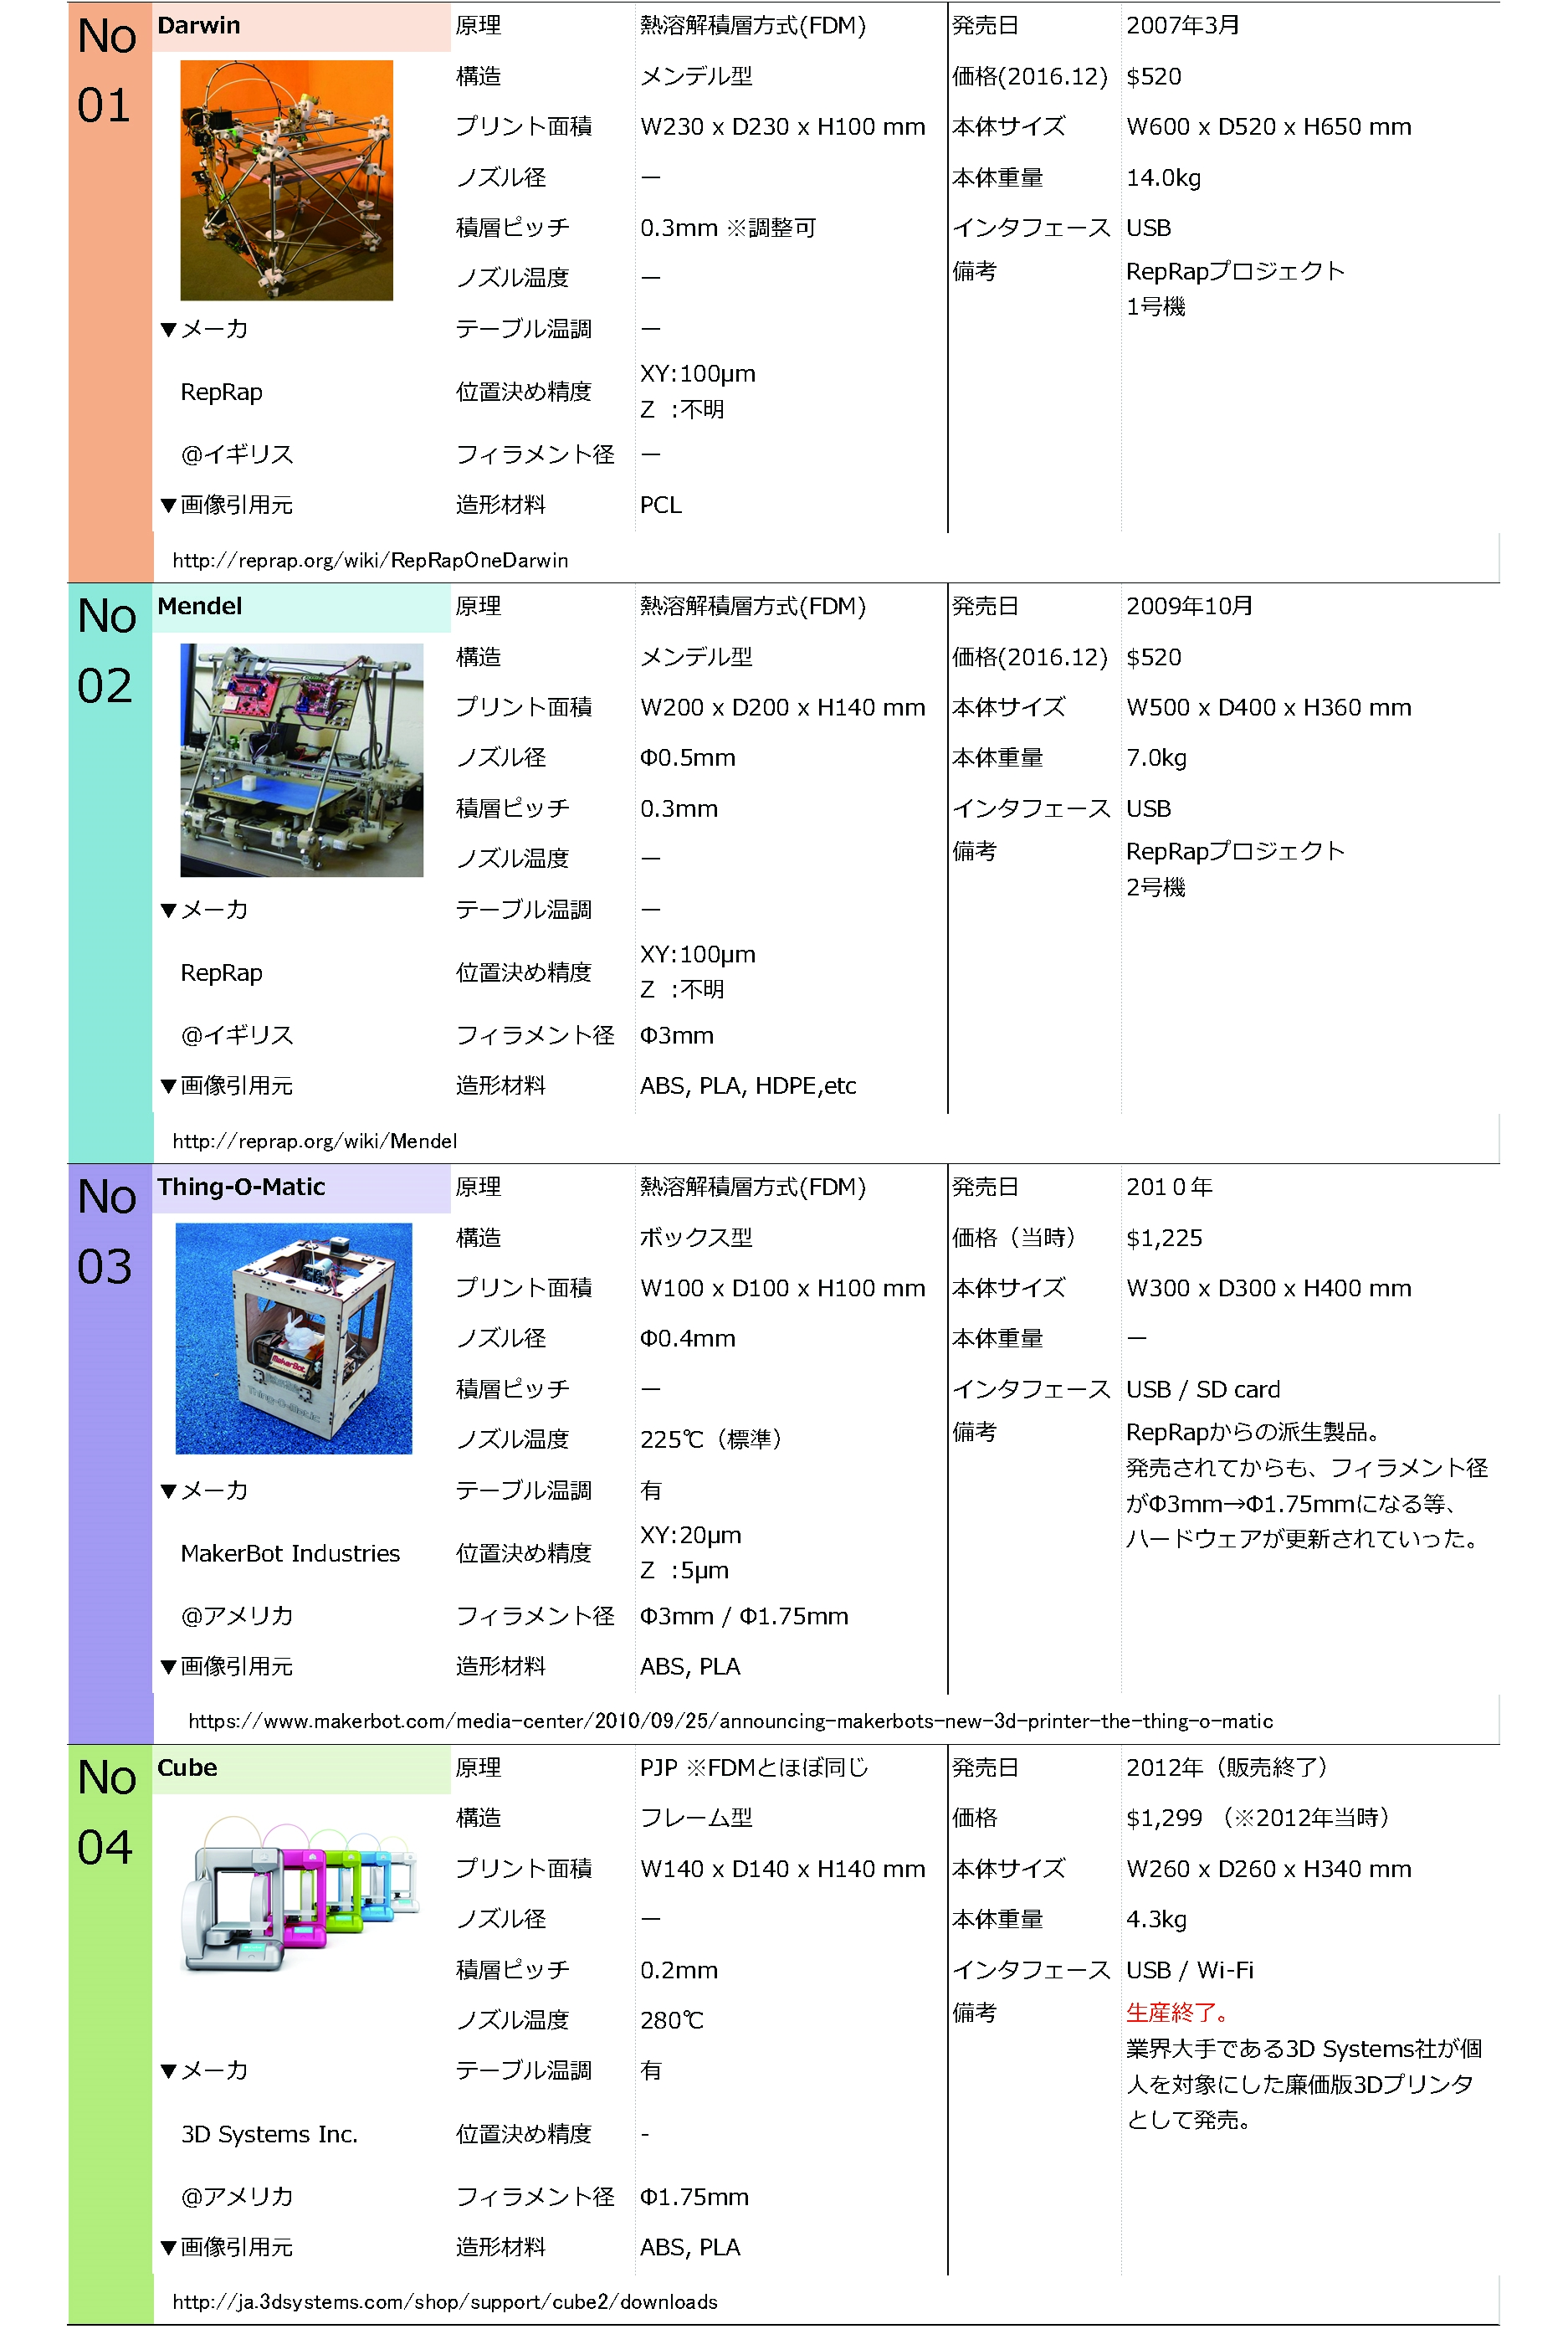
\includegraphics[width=380pt]{fig/fig24_cmyk.jpg}
\caption{3Dプリンタ一覧-1}
\label{fig24}
\end{figure}

\begin{figure}[htbp]
\centering
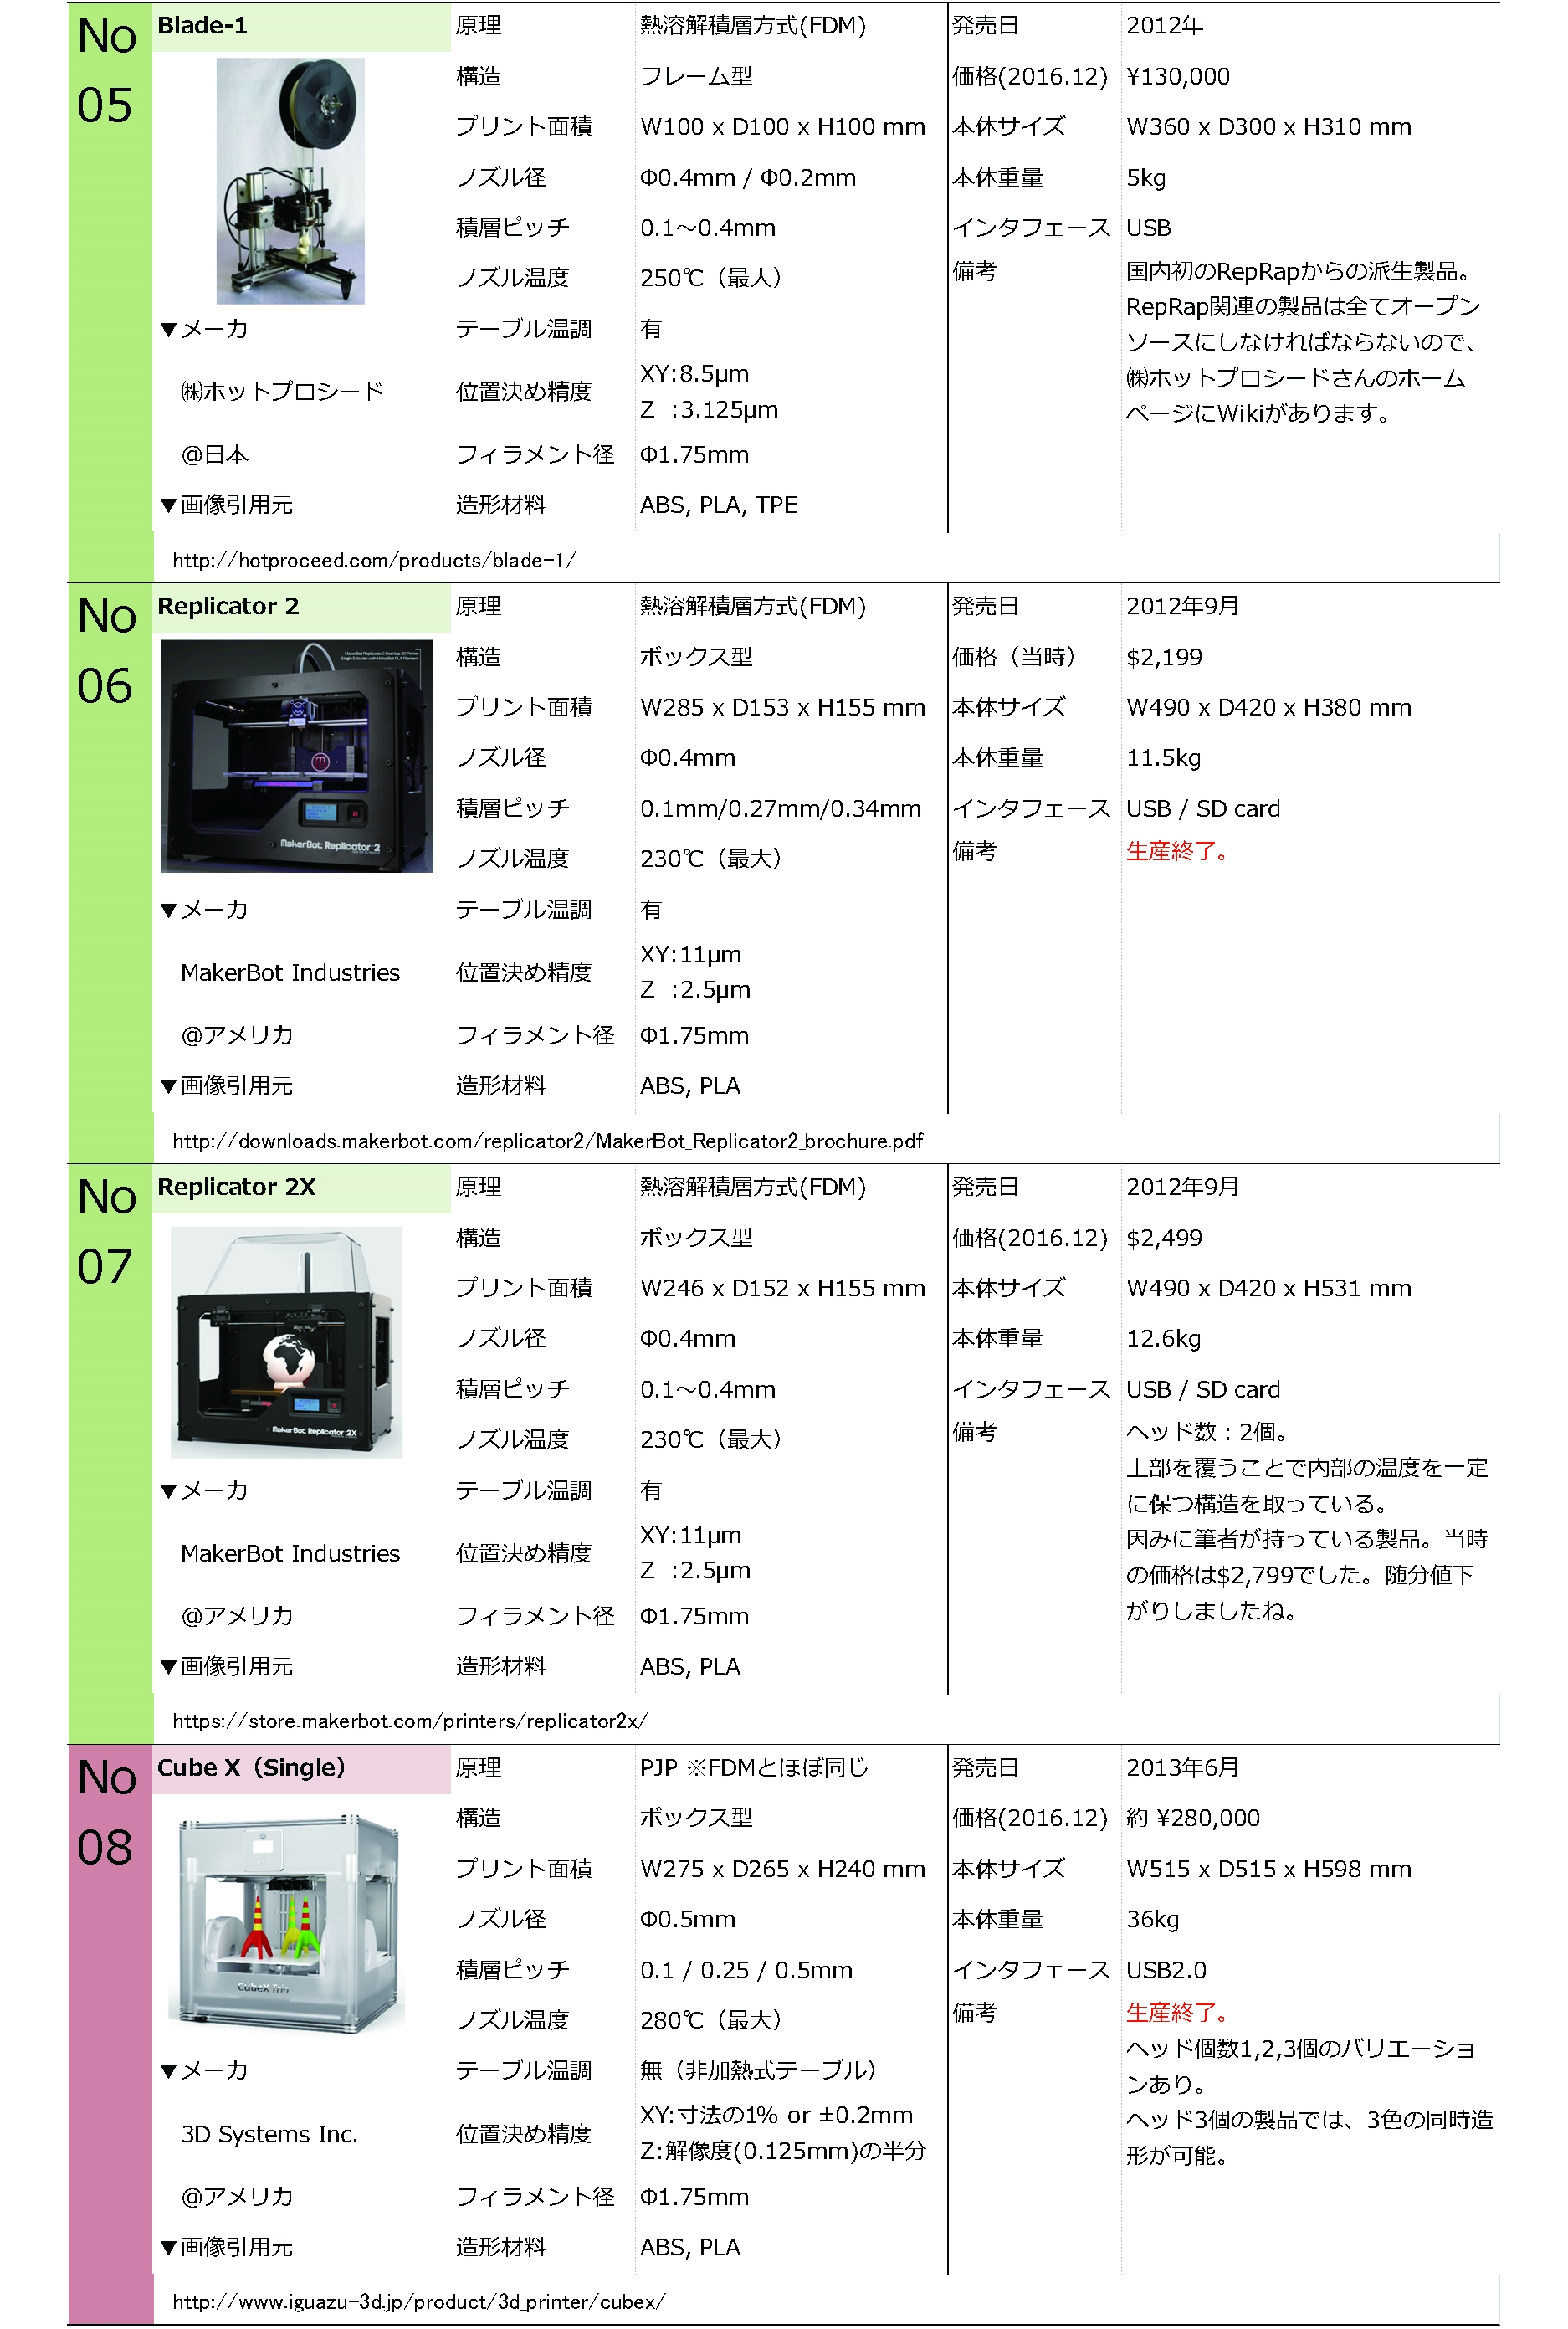
\includegraphics[width=380pt]{fig/fig25_cmyk.jpg}
\caption{3Dプリンタ一覧-2}
\label{fig25}
\end{figure}

\begin{figure}[htbp]
\centering
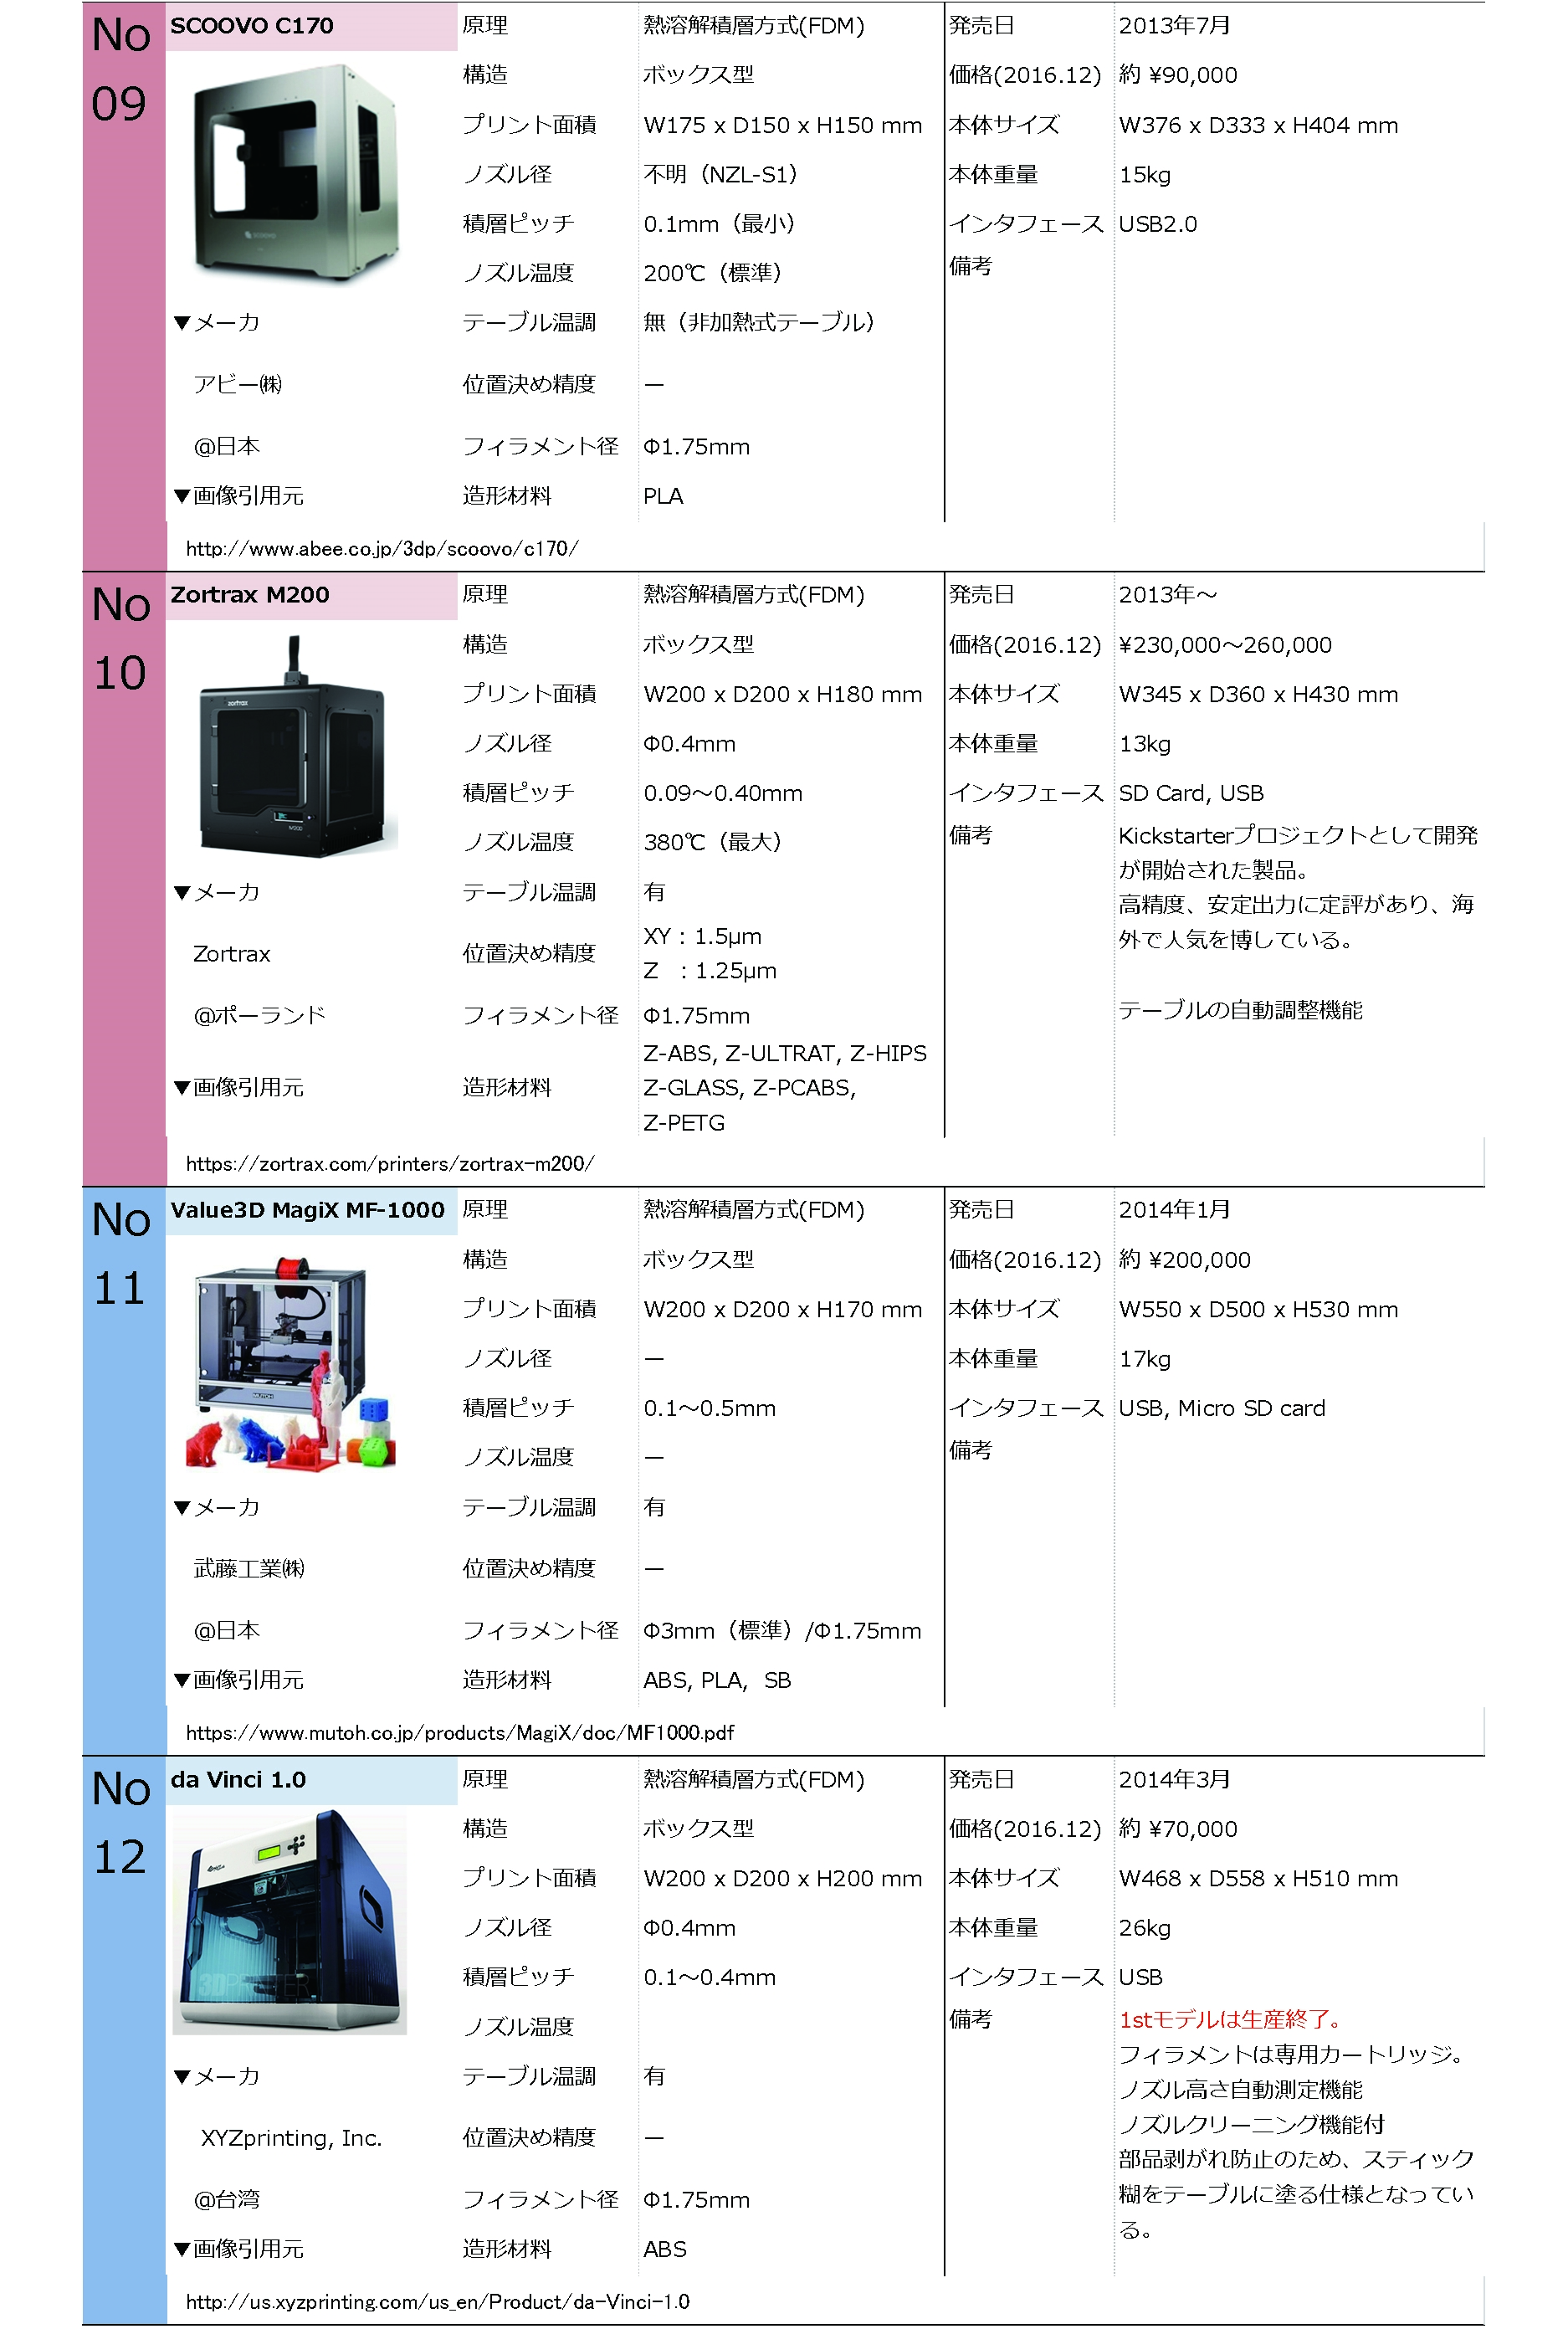
\includegraphics[width=380pt]{fig/fig26_cmyk.jpg}
\caption{3Dプリンタ一覧-3}
\label{fig26}
\end{figure}

\begin{figure}[htbp]
\centering
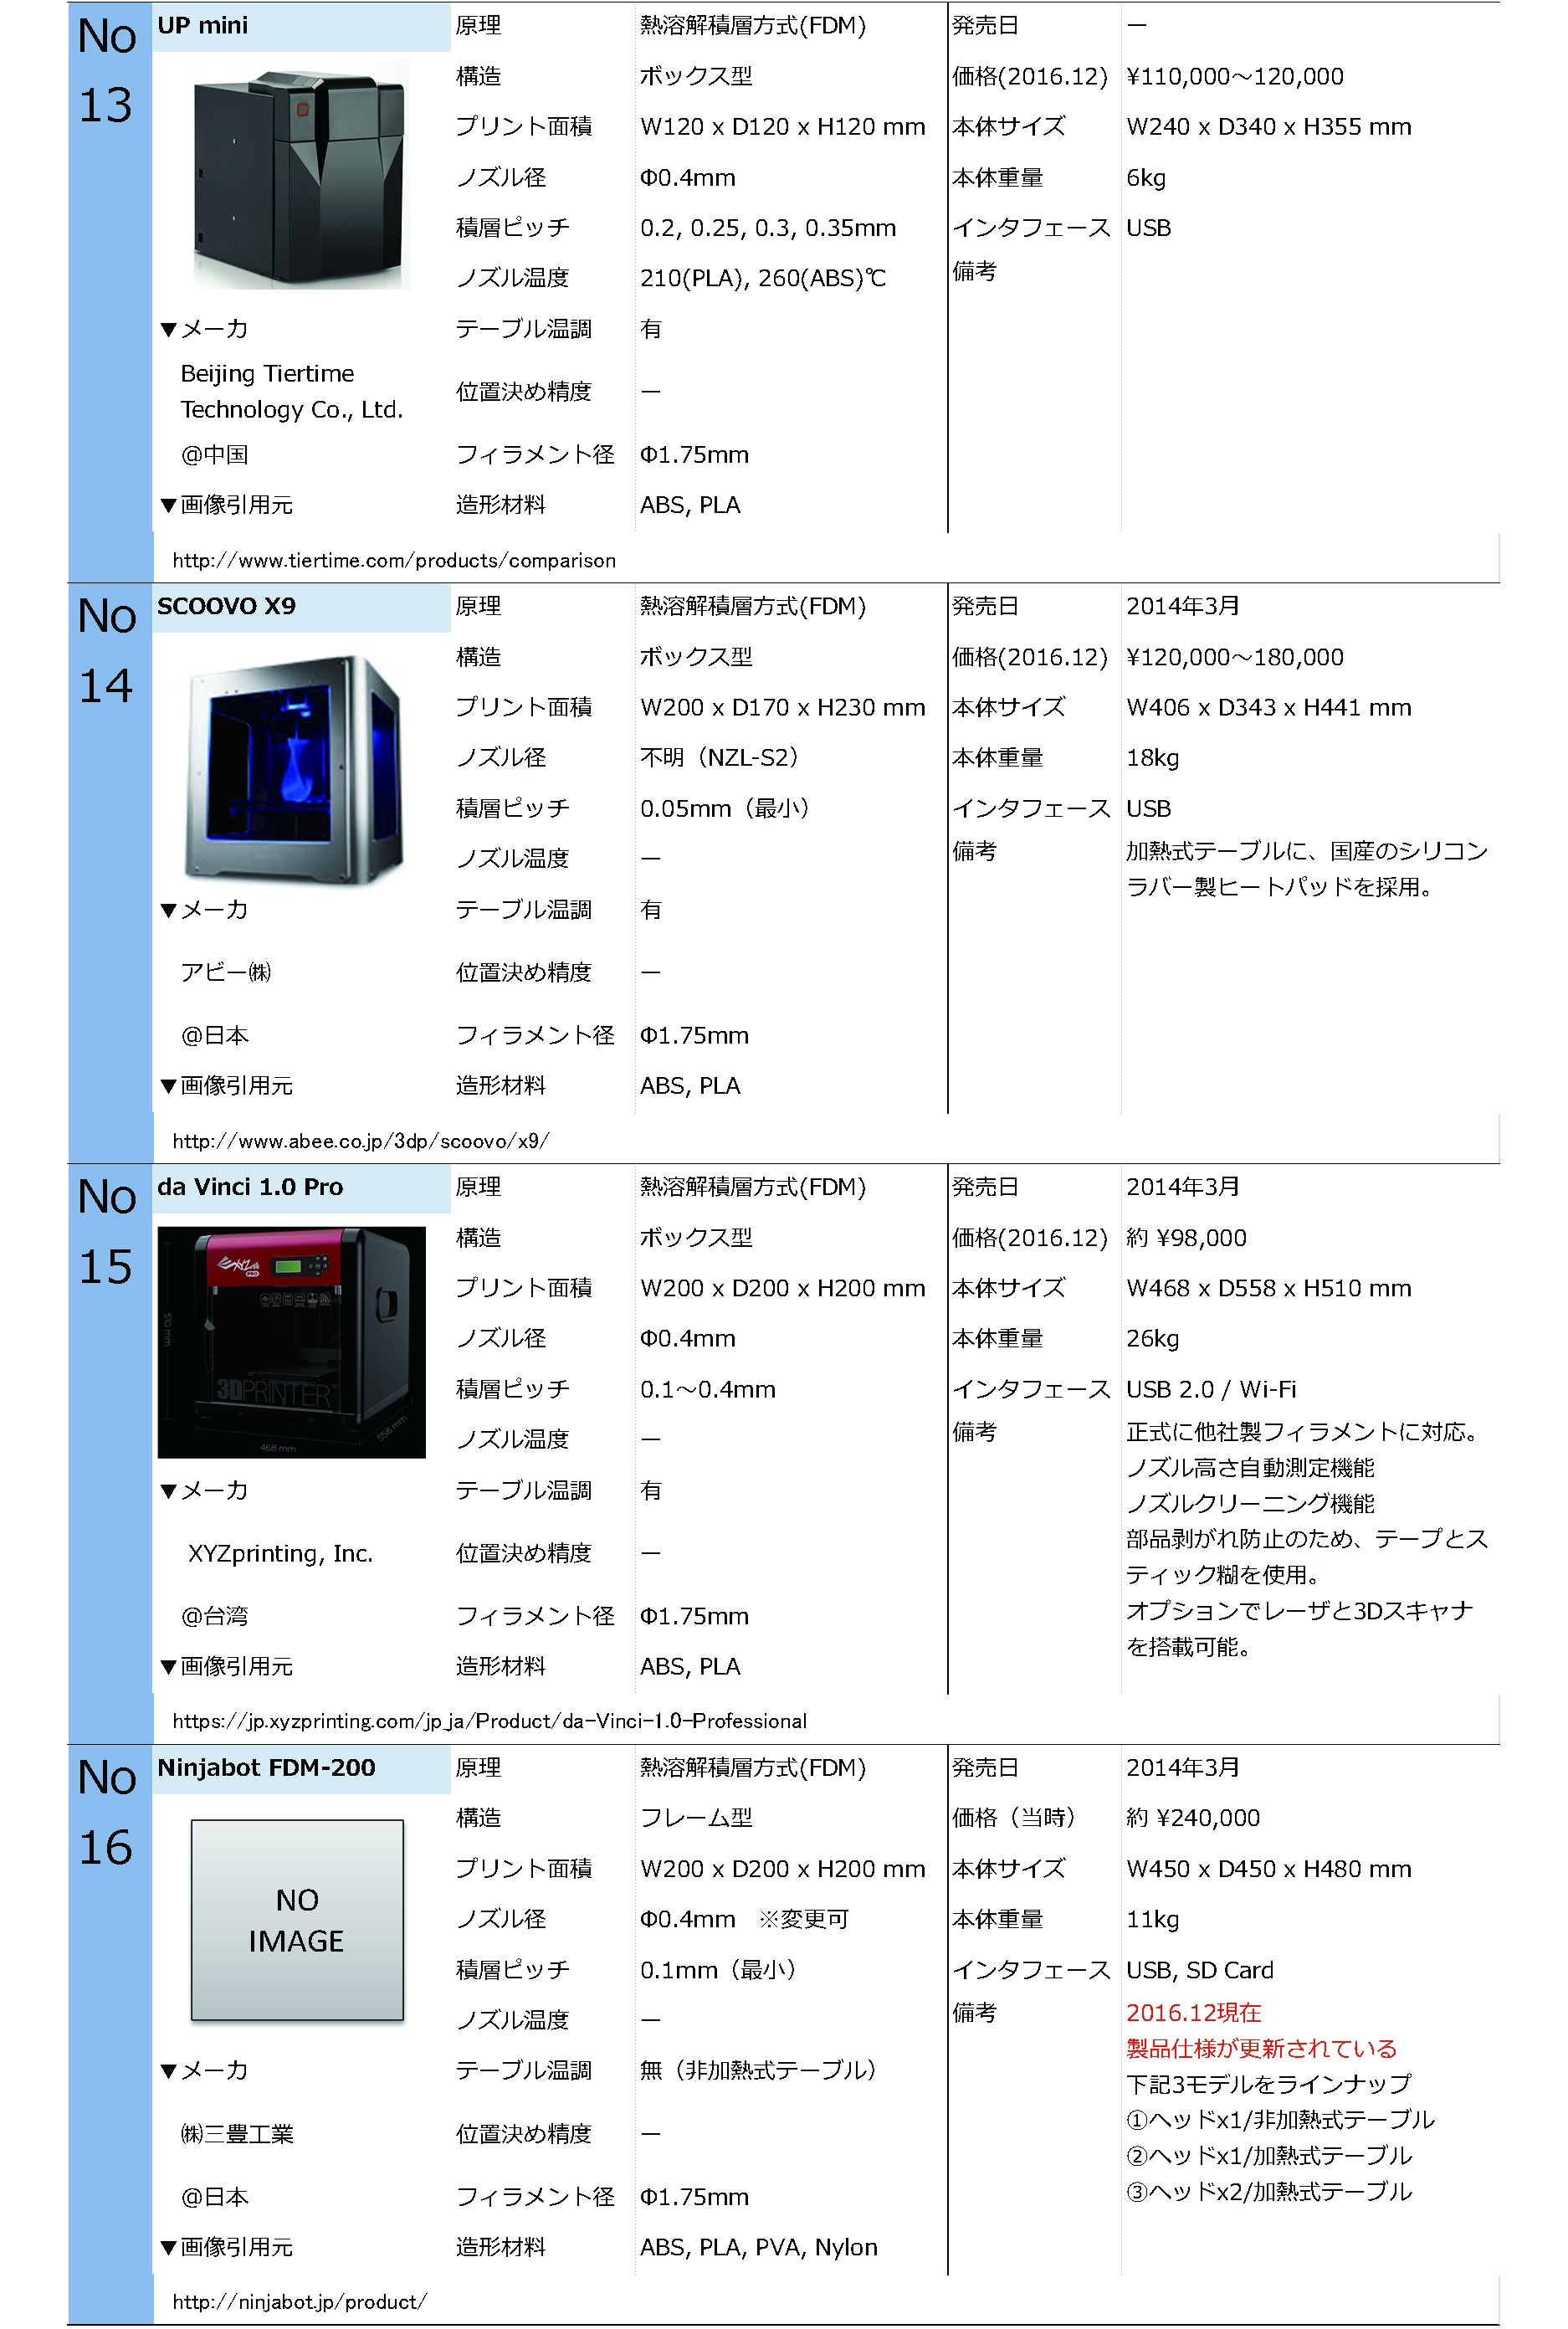
\includegraphics[width=380pt]{fig/fig27_cmyk.jpg}
\caption{3Dプリンタ一覧-4}
\label{fig27}
\end{figure}

\begin{figure}[htbp]
\centering
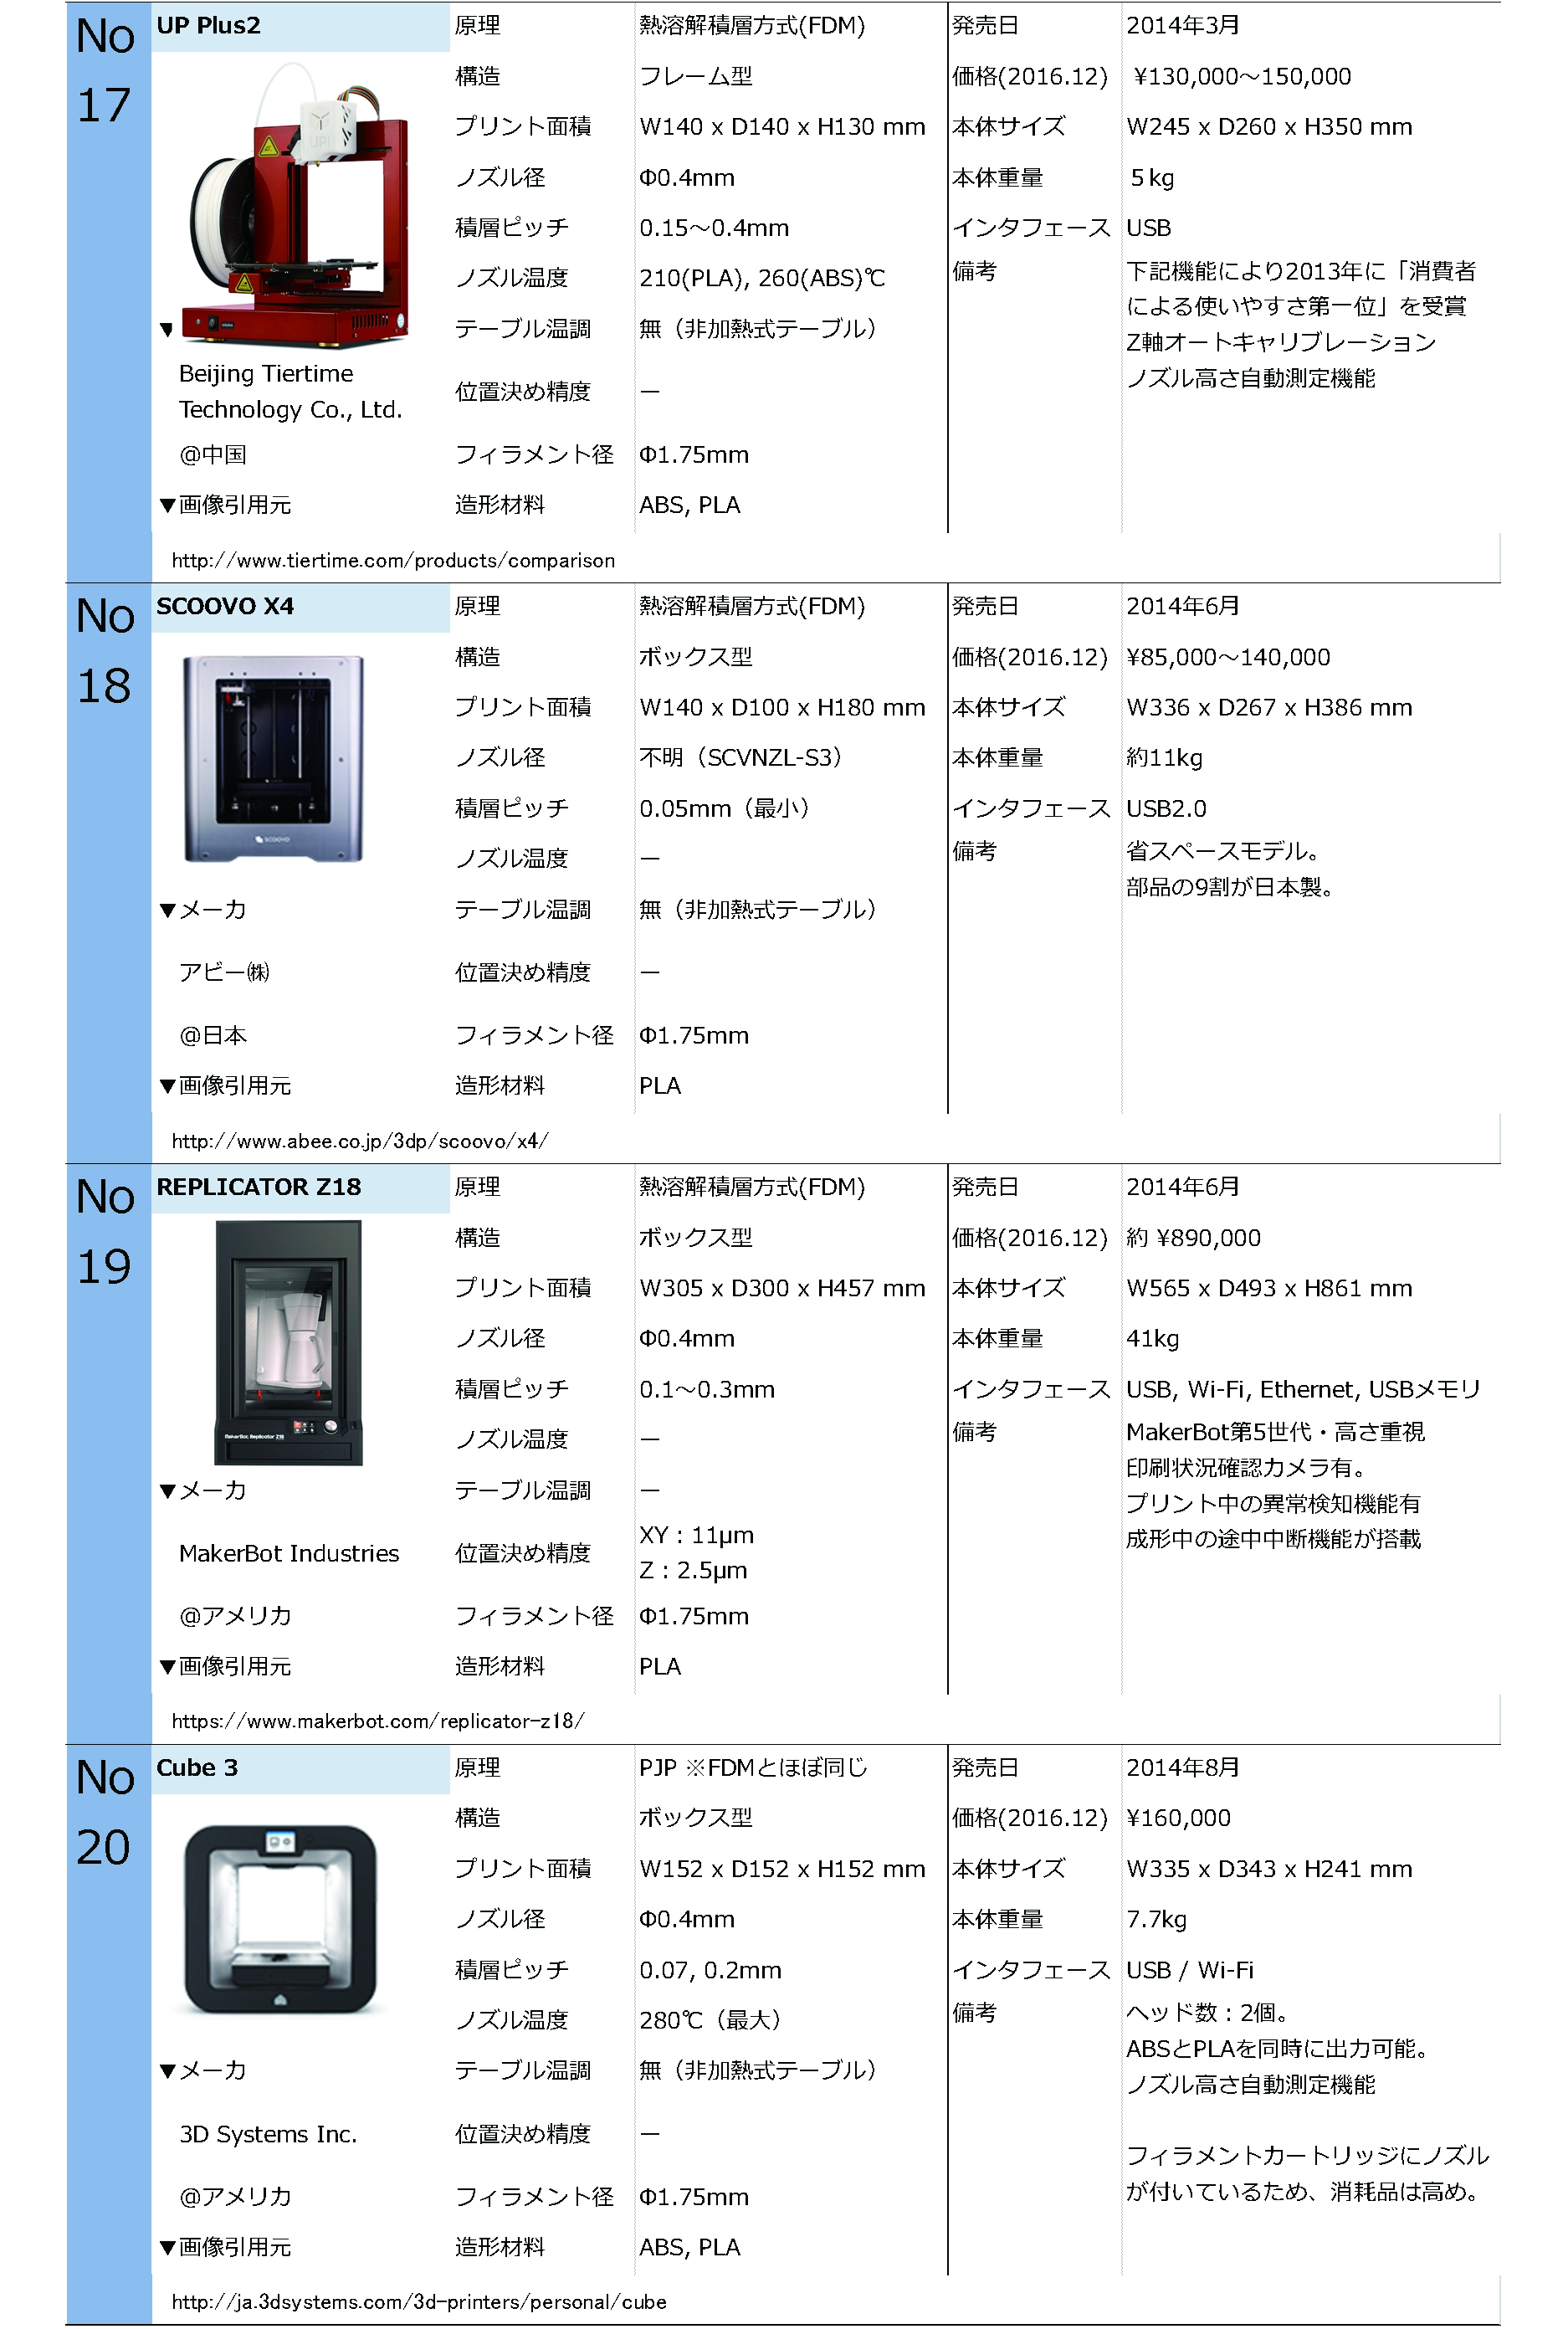
\includegraphics[width=380pt]{fig/fig28_cmyk.jpg}
\caption{3Dプリンタ一覧-5}
\label{fig28}
\end{figure}

\begin{figure}[htbp]
\centering
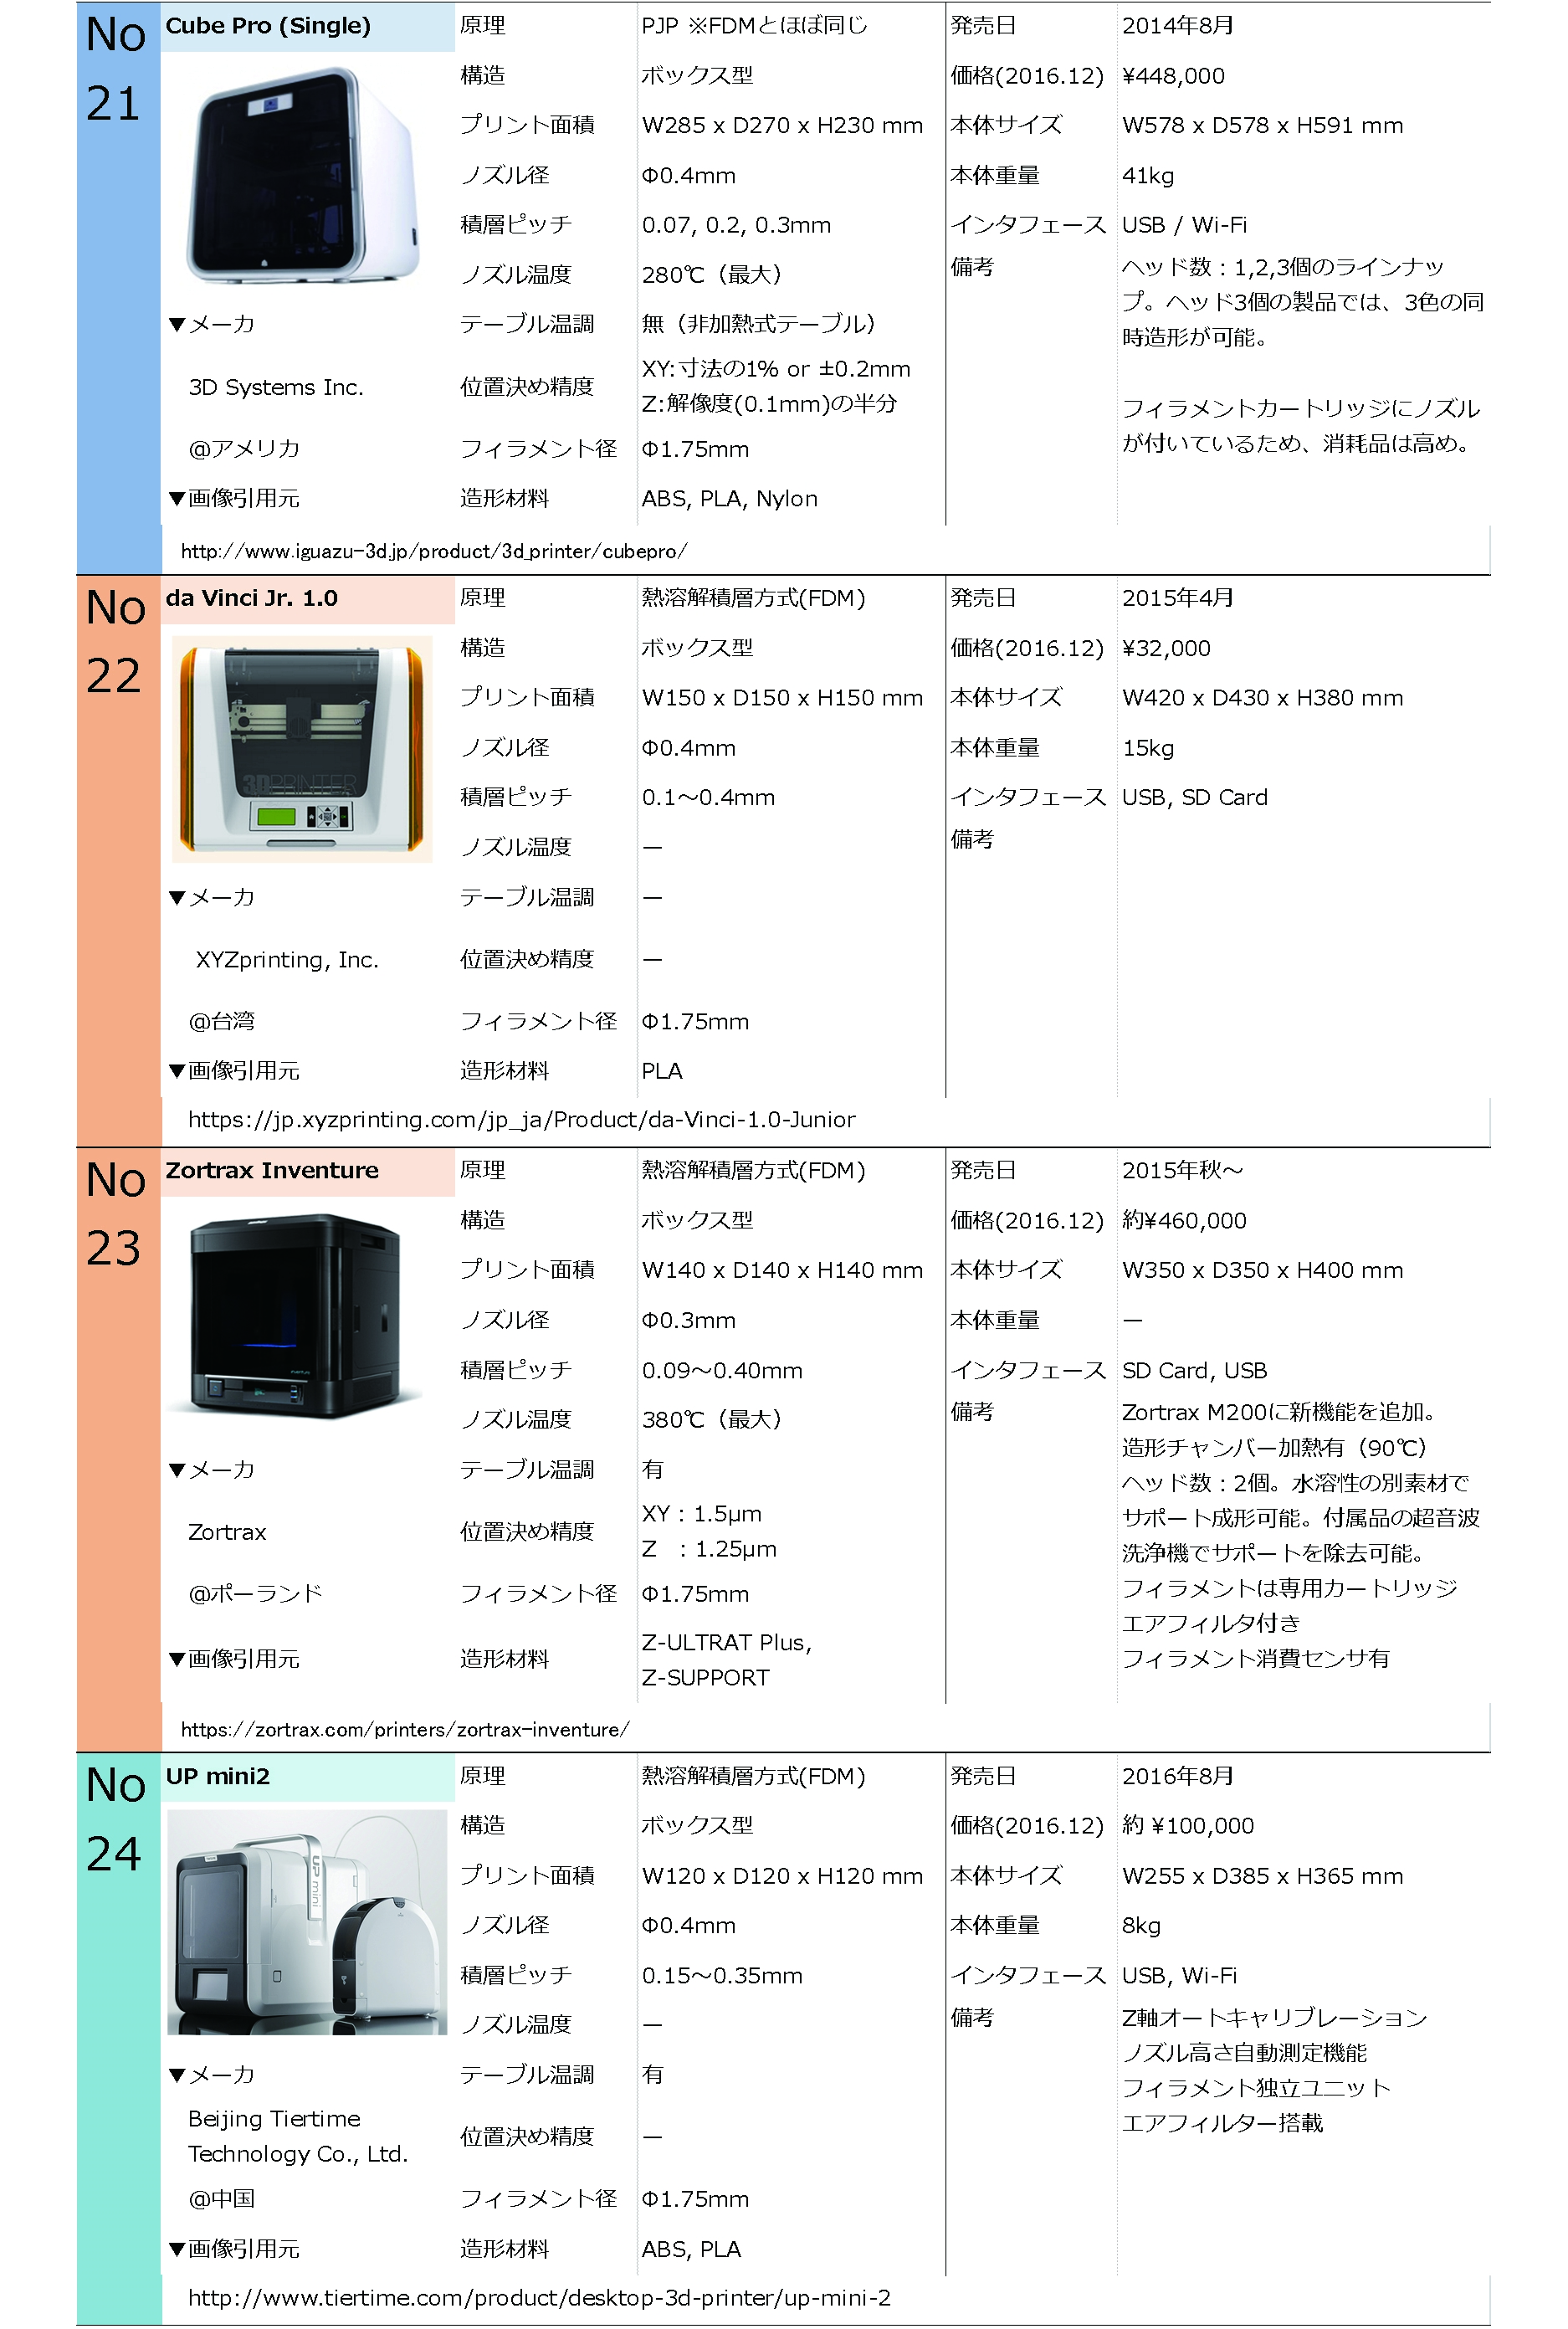
\includegraphics[width=380pt]{fig/fig29_cmyk.jpg}
\caption{3Dプリンタ一覧-6}
\label{fig29}
\end{figure}

\begin{figure}[htbp]
\centering
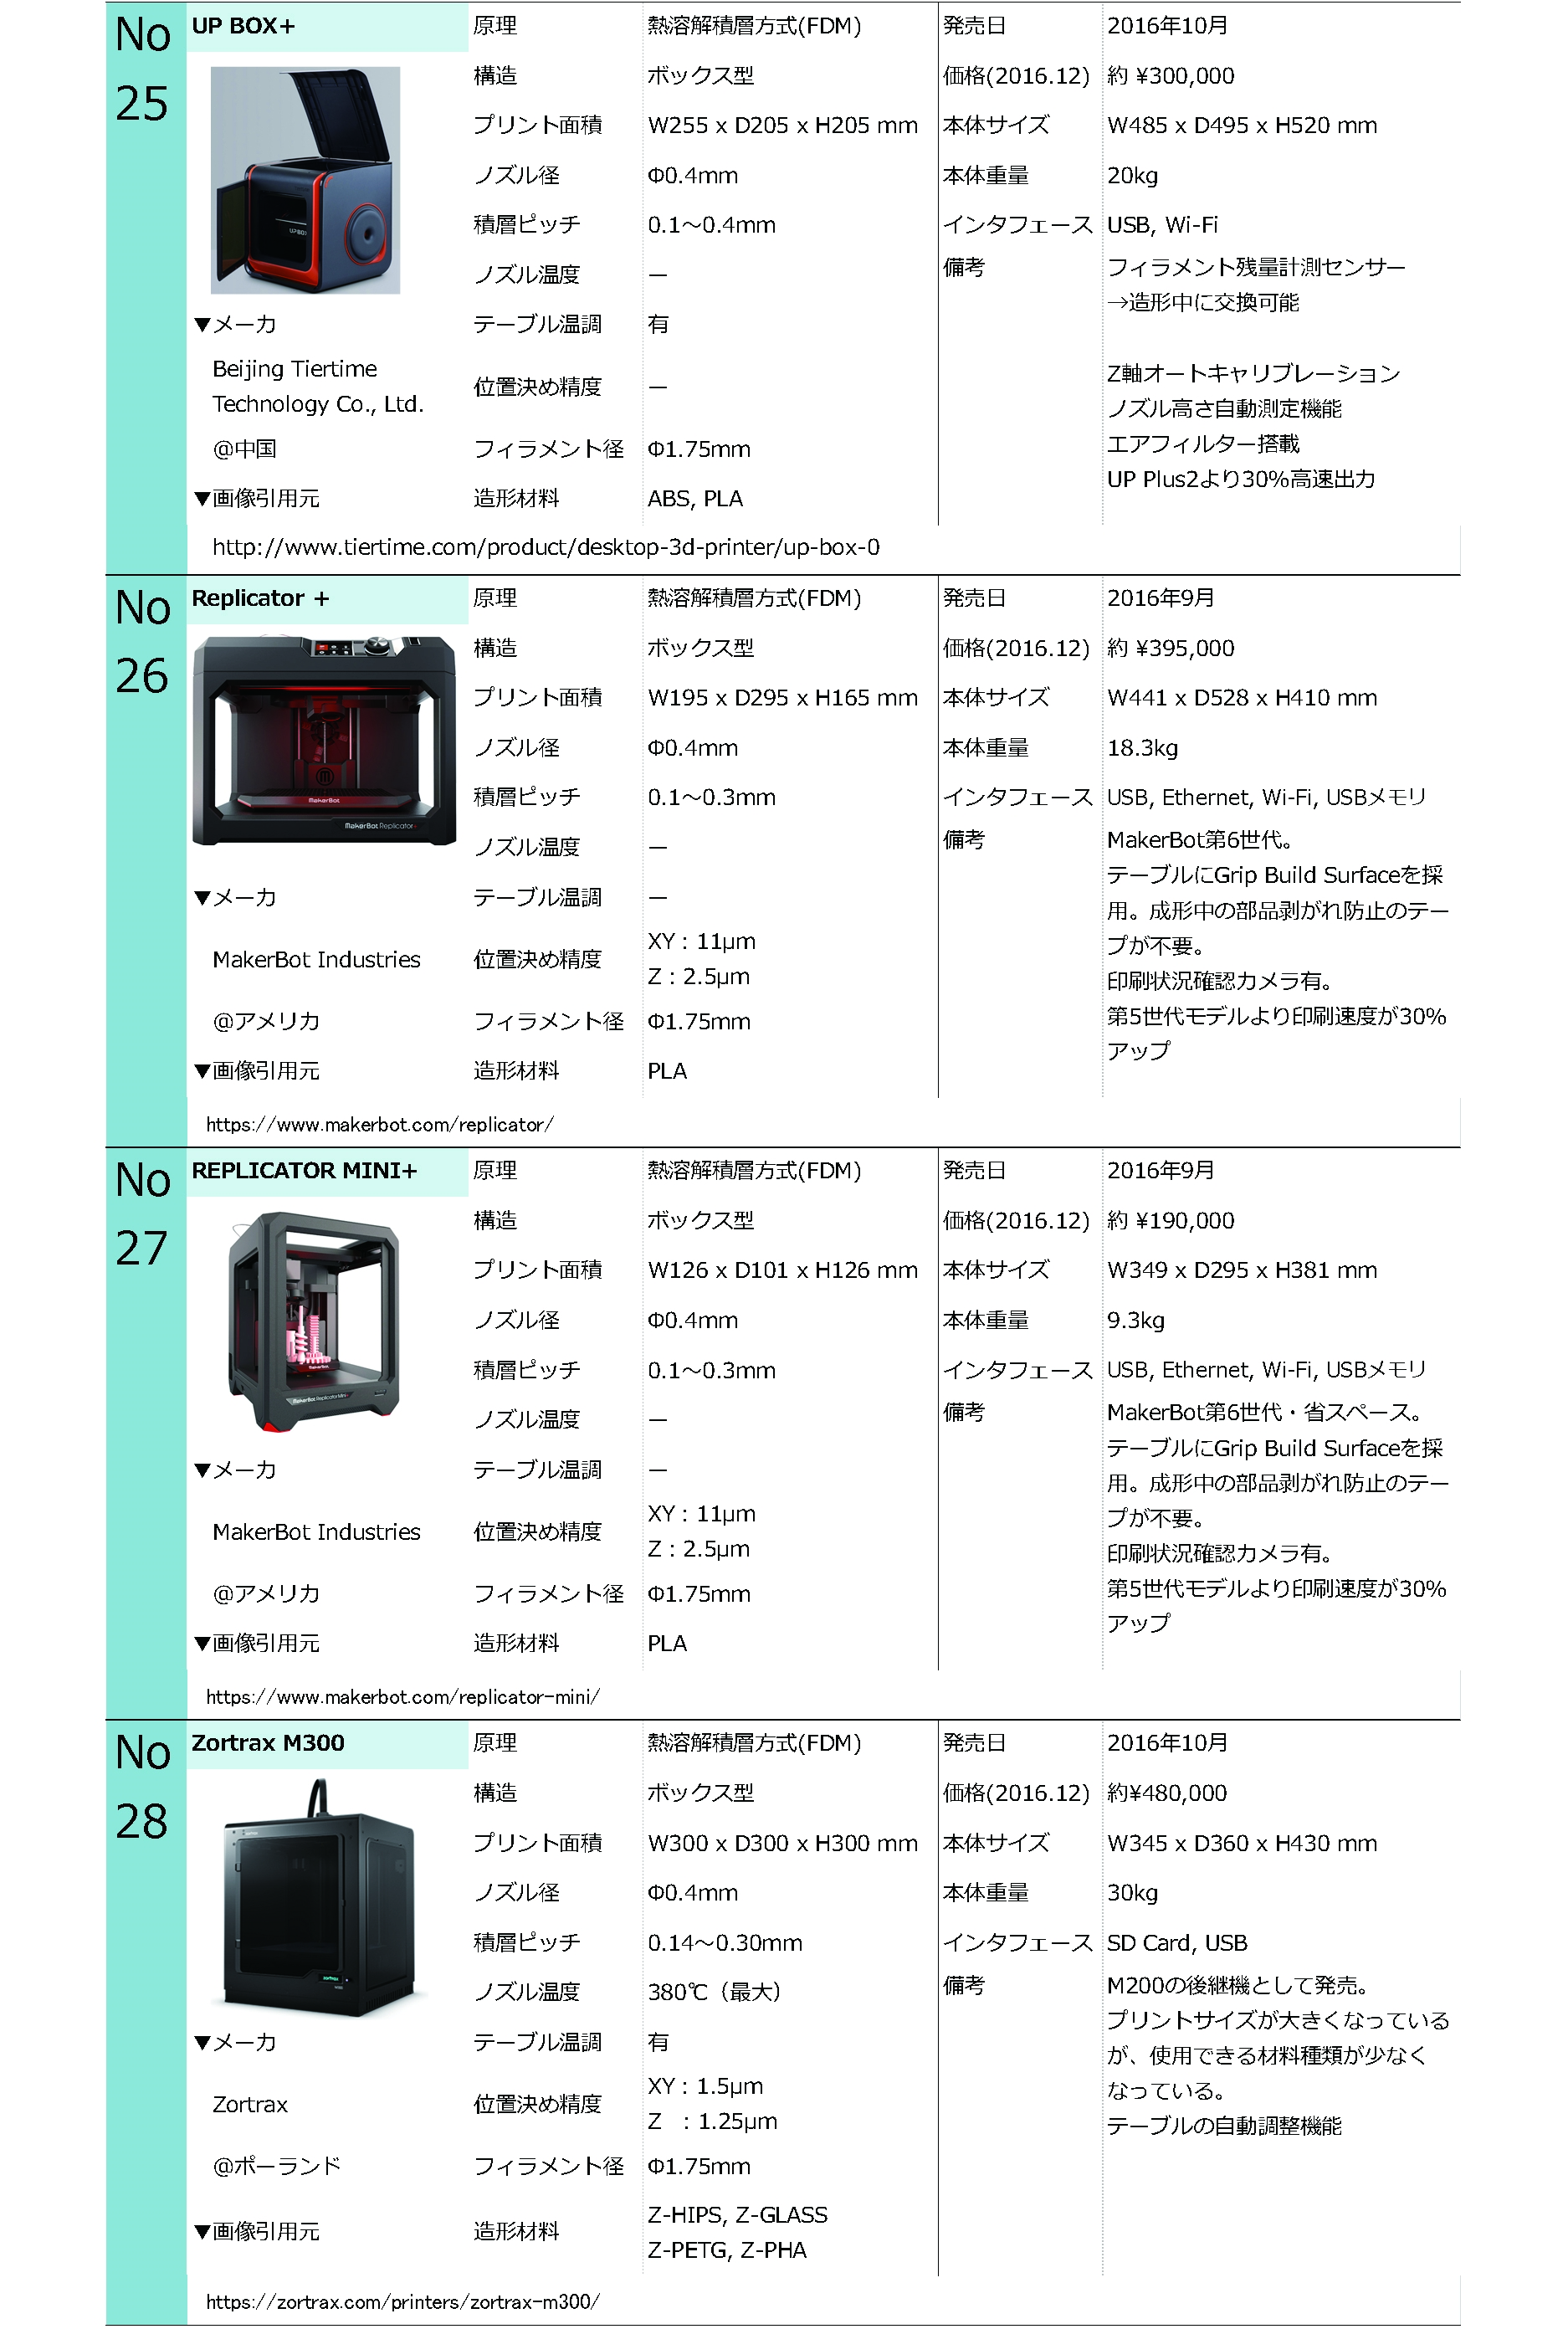
\includegraphics[width=380pt]{fig/fig30_cmyk.jpg}
\caption{3Dプリンタ一覧-7}
\label{fig30}
\end{figure}
